%Author: Hendrik Klug
%template taken from Niklaus Messerli 's Biomedical Imaging formula sheet
%to be printed on A4 borderless with 2 pages on one side


\documentclass[9pt]{article}
\usepackage[utf8]{inputenc}
\usepackage{lastpage}
\usepackage{amsmath}
\usepackage{amssymb}
\usepackage{dsfont}
\usepackage{array}
\usepackage{fancyhdr}
\usepackage[table]{xcolor}
\usepackage{xspace}
\usepackage{graphicx}
\usepackage{float}
\usepackage{comment}

\usepackage{titlesec}
\usepackage{wrapfig}
\usepackage{mhchem}
\usepackage{multicol}
\usepackage{color}
\usepackage{siunitx}
\usepackage{physics}
\usepackage{mathtools}

% no paragraph indentation
\setlength\parindent{0pt}
\setlength{\parskip}{0pt}
\setlength{\parsep}{0pt}
\setlength{\headsep}{0pt}
\setlength{\topskip}{0pt}
\setlength{\topmargin}{0pt}
\setlength{\topsep}{0pt}
\setlength{\partopsep}{0pt}
\definecolor{formula}{RGB}{240,248,255}

%\usepackage[a4paper, lmargin=0.3cm,rmargin=0.3cm,tmargin=0.5cm,bmargin=0.5cm]{geometry}
\usepackage[a4paper, lmargin=0.3cm,rmargin=0.3cm,tmargin=0.5cm,bmargin=0.2cm]{geometry}

\definecolor{lightgrey}{gray}{0.9}
\definecolor{lgrey}{rgb}{0.9,0.9,0.9}
\newcommand{\grey}[1]{\setlength{\fboxsep}{0pt}\colorbox{lightgrey}{#1}}

% reduce space after subsubsection title
%\titlespacing*{\subsubsection}{0pt}{3.25ex plus 0ex minus .2ex}{0.5ex plus 0ex}
\usepackage{titlesec}
\titlespacing{\section}{0pt}{*0}{*0}
\titlespacing{\subsection}{0pt}{*0}{*0}
\titlespacing{\subsubsection}{0pt}{*0}{6pt}

\titleformat{\subsubsection}[runin]{\normalfont\bfseries}{\thesubsubsection}{3pt}{}[:]


% for table formatting
\def\arraystretch{1.3}
\definecolor{lgrey}{rgb}{0.9,0.9,0.9}
\newcolumntype{L}[1]{>{\raggedright\let\newline\\\arraybackslash\hspace{0pt}}m{#1}}
\newcolumntype{C}[1]{>{\centering\let\newline\\\arraybackslash\hspace{0pt}}m{#1}}
\newcolumntype{R}[1]{>{\raggedleft\let\newline\\\arraybackslash\hspace{0pt}}m{#1}}

% page header, no footer
\pagestyle{fancy}
%\lhead{Formulary Biomedical Imaging}
\lhead{}
%\chead{\thepage\ of \pageref{LastPage}}
\chead{}
%\rhead{HS2018}
\rhead{}
\fancyfoot{}
\renewcommand{\headrulewidth}{0.4pt}
\setlength{\headheight}{0pt}
\setlength{\headsep}{15pt}

  \providecommand{\D}{\vec{D}} 
  \providecommand{\E}{\vec{E}} 
  \providecommand{\B}{\vec{B}} 
  \providecommand{\B}{\vec{B}}
  \providecommand{\A}{\vec{A}}
  \providecommand{\nv}{\vec{\nabla}}
  \providecommand{\e}{\varepsilon}

% equation box        
\newcommand{\eqbox}[1]{\fcolorbox{black}{formula}{\hspace{0.5em}$\displaystyle#1$\hspace{0.5em}}}

% shortcuts
\newcommand{\dif}{\mathrm{d}}
\newcommand{\del}{\partial}
\newcommand{\fcal}{\mathcal{F}}
\newcommand{\TODO}{\colorbox{lime}{TODOTODOTODO}}

% danger symbol
\newcommand*{\TakeFourierOrnament}[1]{{%
		\fontencoding{U}\fontfamily{futs}\selectfont\char#1}}
\newcommand*{\danger}{\TakeFourierOrnament{66}}


\begin{document}

\fontsize{9.2pt}{10pt}\selectfont


\begin{multicols}{2}

\section{Introduction to biomedical Sensors}
	\textbf{Biosensor:}
	\begin{itemize}
	\item A device that detects, records and transmits information regarding a physiological change or process.
	\item A device that uses biological materials to monitor the presence of various chemicals in a substance
	\end{itemize}
	\textbf{Bioelectronics:}
	\begin{itemize}
	\item The application of the principles of electronics to biology and medicine.
	\item The study of the role of intermolecular electron transfer in physiological processes.
	\end{itemize}
	
\textbf{Biosensor Principle:} Biosample $\rightarrow$ Element recognition $\rightarrow$ Transducer $\rightarrow$ Signal Processing $\rightarrow$ Signal\\
Can capture the wanted molecules with antibodies that were previously created by rats.
	\subsection{Current Problems:}
	\textbf{Sample Size:} Tumor is curable when it is really small, but hard to find without big Aufwand\\
	\textbf{Sensitivity:} All biosensing techniques are limited by the non-specific interactions.\\
	\textbf{Specificity}\\
	\textbf{Continous Monitoring:} $\rightarrow$ need noninvasive sensors
	\subsection{Receptor binding:}
	$k_{on}[A][R]=k_{off}[AR]$ $\rightarrow$ \eqbox{K_a=\frac{k_{on}}{k_{off}}=\frac{[AR]}{[A][R]}} (equilibrium constant)\\
	When half of the receptors are occupied, $[AR] = [R]$ $\rightarrow$ Good way to measure quality of sensor\\
	\textbf{Non-Specific Binding:} other molecules that bind to the same receptor as the analyte. This is a fundamental limit related to the lack of receptors with high-affinity. (big net analogy when specific binding is small compared to non-specific: capture tons of fish, hard to find nemo)\\
	The \textbf{limit of detection} (LOD) is defined as the concentration at which the signal $S_{LOD} = S_0 + 3\cdot \ noise$, with $S_0$ the signal without analyte. For low analyte concentration the curve signal/(analyte concentration) is a straight line:\\
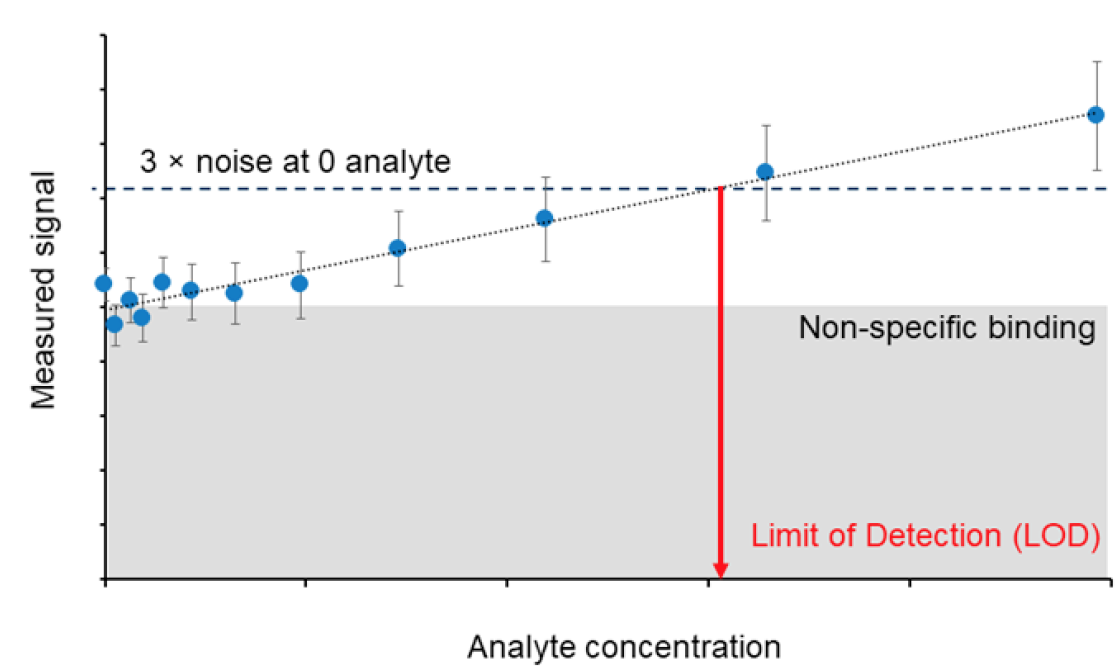
\includegraphics[scale=0.3]{Images/LOD.png} $\dfrac{dS}{d[A]}= \dfrac{3\cdot noise}{LOD}$

\section{Fundamentals of Microscopy}
\subsection{Maxwells equations}
						\textbf{Continuity Equation: }$ \vec{\nabla} \cdot \vec{j}(\textbf{r},t) + \frac{\partial \rho(\textbf{r},t) }{\partial t}$\\
					\textbf{Gauss-Law: } $\vec{\nabla} \cdot \vec{D}(\textbf{r},t)=\rho(\textbf{r}, t)$\\
					\textbf{Farraday's Law: }
					$ \vec{\nabla} \times \vec{E} (\textbf{r},t)= -\frac{\partial}{\partial t}\vec{B}(\textbf{r},t) $\\
					\textbf{Ampere/Oersted }
					$ \vec{\nabla} \times \vec{H} (\textbf{r},t) = \frac{\partial}{\partial t}\vec{D}(\textbf{r},t)+\vec{j}(\textbf{r},t) $\\
					\textbf{No magnetic Monopoles: }
					$ \vec{\nabla} \cdot \vec{B} (\textbf{r},t)=0  $
\subsubsection{Monochromatic fields}.\\
\textbf{Gauss-Law: }
					$\vec{\nabla} \cdot \vec{D}(\textbf{r})=\rho(\textbf{r})$\\
					\textbf{Farraday's Law: }
					$\vec{\nabla} \times \vec{E} (\textbf{r})= -i \omega \vec{B}(\textbf{r}) $\\
					\textbf{Ampere/Oersted:  }
					$\vec{\nabla} \times \vec{H} (\textbf{r}) = i\omega \vec{D}(\textbf{r})+\vec{j}(\textbf{r}) $
\subsubsection{The wave equation}.\\
	$\nv \times \nv \times \E + \frac{1}{c^{2}}\frac{\partial^{2}\E}{\partial t^{2}} = -\mu_{0} \frac{\partial}{\partial t }(\vec{j}+ \frac{\partial P}{\partial t}+ \nv \times M)$\\
					$\nv \times \nv \times \vec{H} + \frac{1}{c^{2}}\frac{\partial^{2}\vec{H}}{\partial t^{2}} = (\nv  \times \vec{j}+ \nv \times \frac{\partial P}{\partial t}+ \frac{1}{c^{2}} \frac{\partial^{2} M}{\partial t^{2}}) $\\
Direction of propagation: $\E \times \B$\\
Velocity: $c \approx 3\cdot 10^8\ m/s$\\
$|\vec{E_0}|=c|\vec{B_0}|$; $ck=\omega$\\
At large distances from the source, a spherical wave may be approximated by a plane wave
\subsection{Reflection $\&$ Refraction of plane waves}
Law of reflection: $\theta _i=\theta _r$\\
Continuity of wavefronts across the boundary: $\lambda _{glass}/sin(\theta _i)=\lambda _{air}/sin(\theta _t)$ $\rightarrow$
Law of refraction (Snell's Law): $n_i sin(\theta _i) = n_t sin(\theta _t)$\\
total reflection for $\theta _i = \theta _c$, with  $sin(\theta _c)=n_t/n_i$\\
$\lambda _{air} = \lambda _{vac}/n_{air}$\\
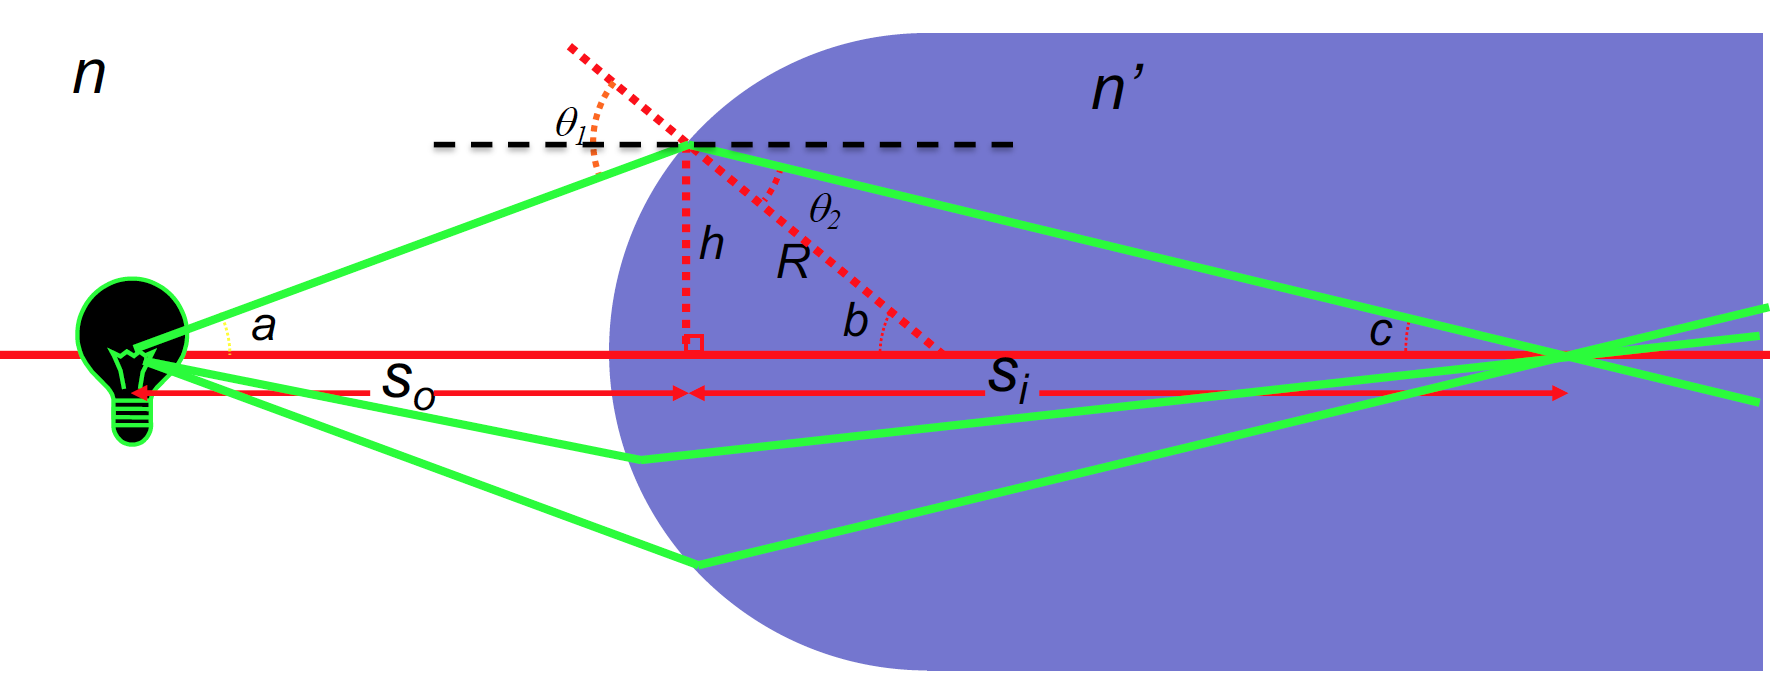
\includegraphics[scale=0.2]{Images/spherical_interfaces.png}\\
$n\ sin(\theta _1)=n'\ sin(\theta _2)$\\
$sin(\theta _1) \approx \sin \alpha + \sin b \approx \frac{h}{s_0}+\frac{h}{R}$\\
$sin(\theta _2) \approx \sin b+ \sin c \approx \frac{h}{R}+\frac{h}{s_i}$\\
$\Rightarrow$ \eqbox{\frac{n}{s_0}+\frac{n'}{s_i}=\frac{(n'-n)}{R}}\\
- Paraxial approx. $\theta \approx \sin \theta \approx \tan \theta$\\
- Thin lens approx: $R << S_0, S_i$\\
- $S_i $ does not depend on the angle\\
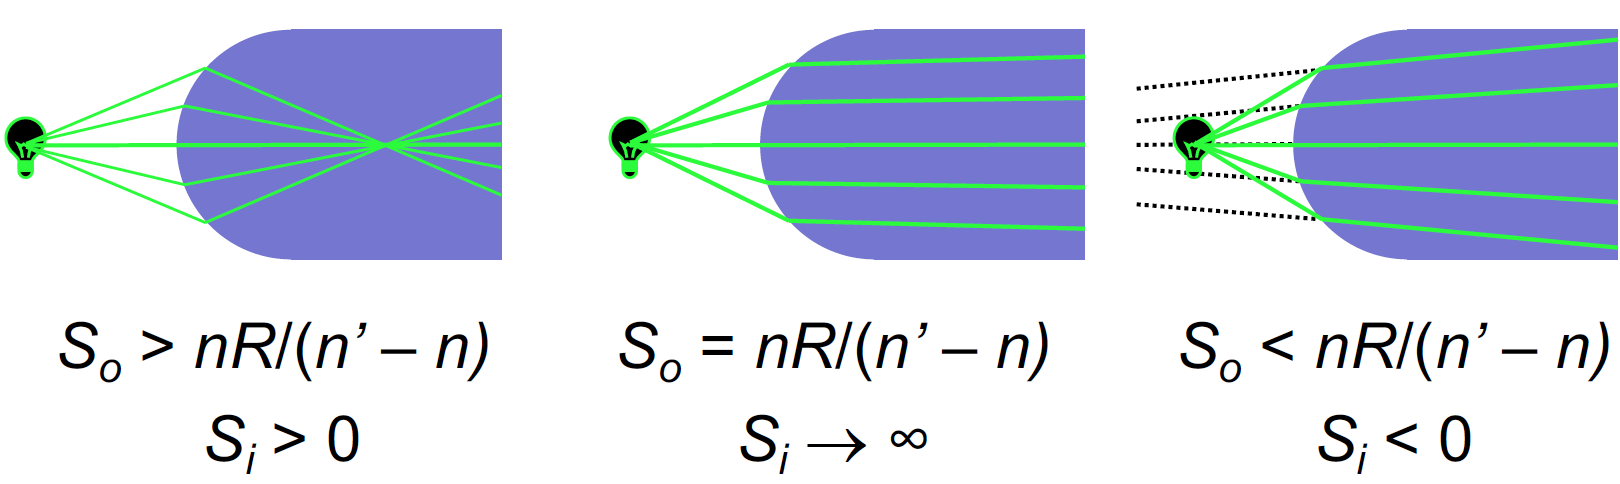
\includegraphics[scale=0.2]{Images/focusing.png}
\subsection{Lenses}
Lens makers' fomrula: \eqbox{\frac{1}{S_0}+\frac{1}{S_i}=\frac{1}{f}=\frac{(n'-n)}{n}(\frac{1}{R_1}-\frac{1}{R_2})}\\
f is the \textbf{focal length}\\
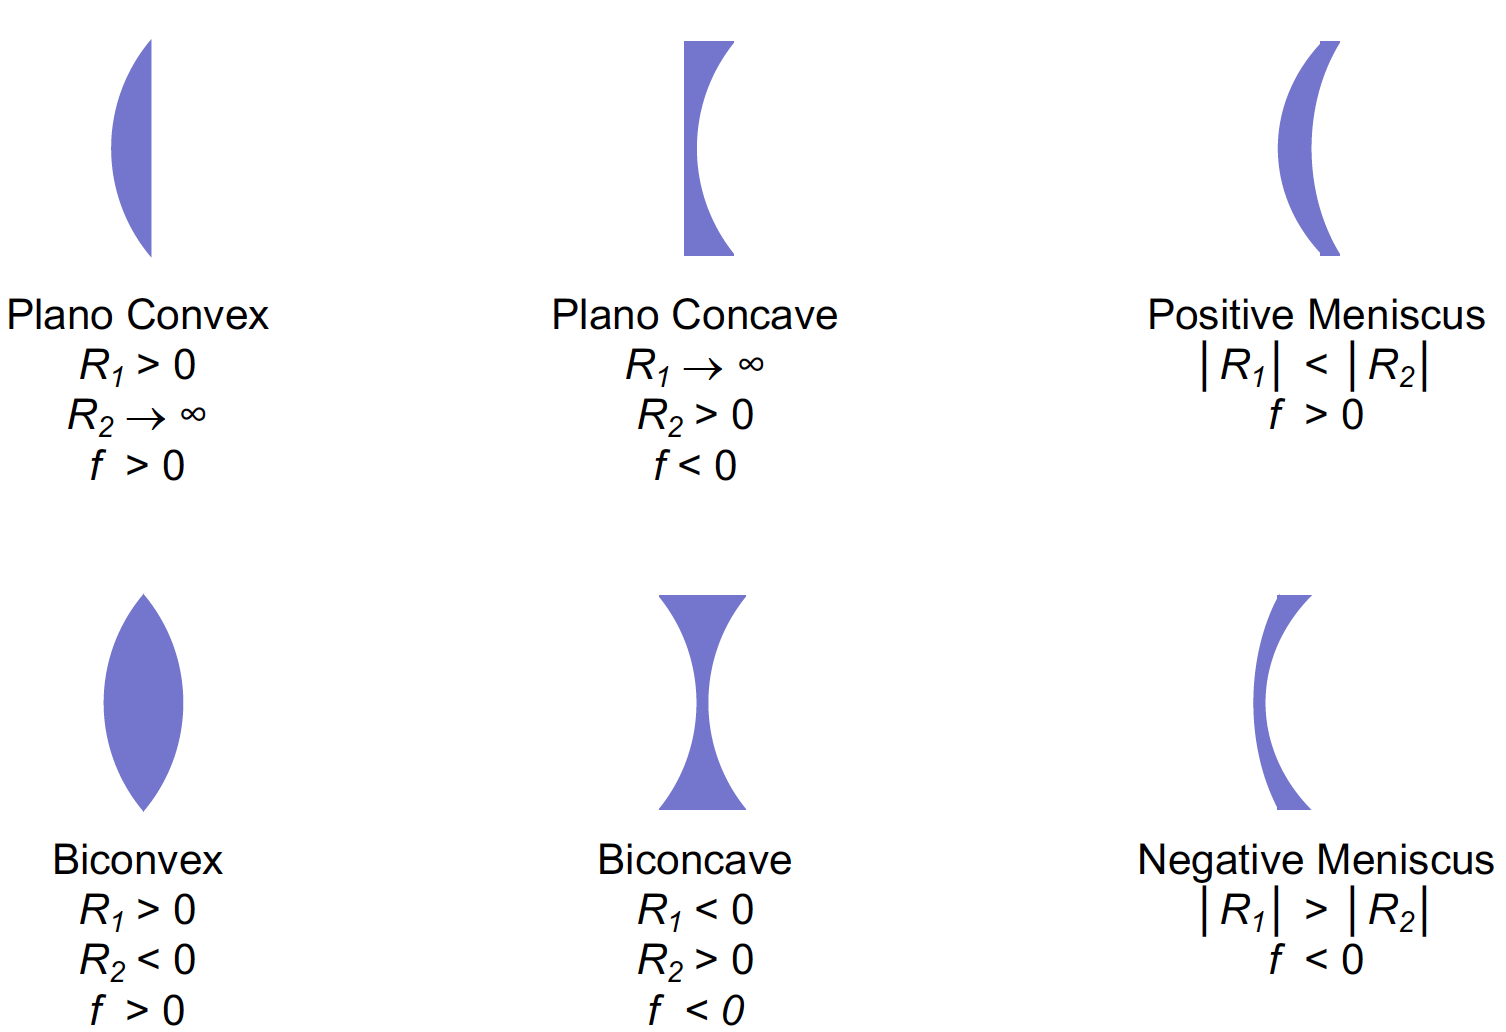
\includegraphics[scale=0.2]{Images/types_of_lenses.png}\\
- Rays passing through the optical
center of a lens continue in a
straight line\\
- Rays traveling parallel to the
optical axis pass through the focal
point after refraction and vice versa\\
- Parallel rays pass through the
same point in the focal plane after
refraction and vice versa\\
\subsubsection{Simple Microscope}.\\
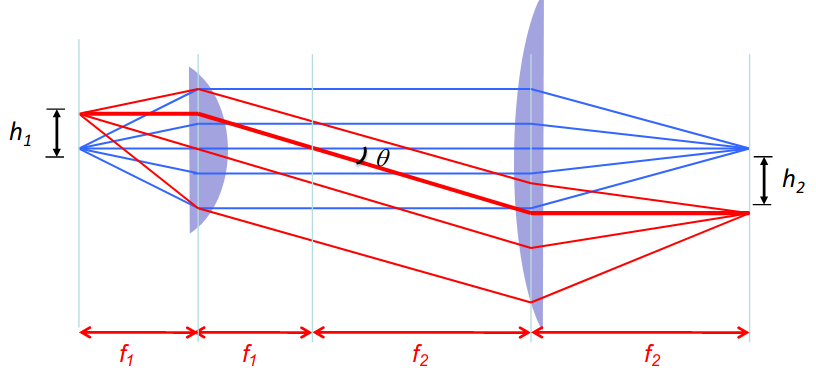
\includegraphics[scale=0.1]{Images/magnification.png} 
Object is magnified by $h_2 /h_1$\\
$h_1=f_1 \sin \theta$ and $h_2=f_2 \sin \theta$ $\Rightarrow M = h_2/h_1=f_2/f_1$\\
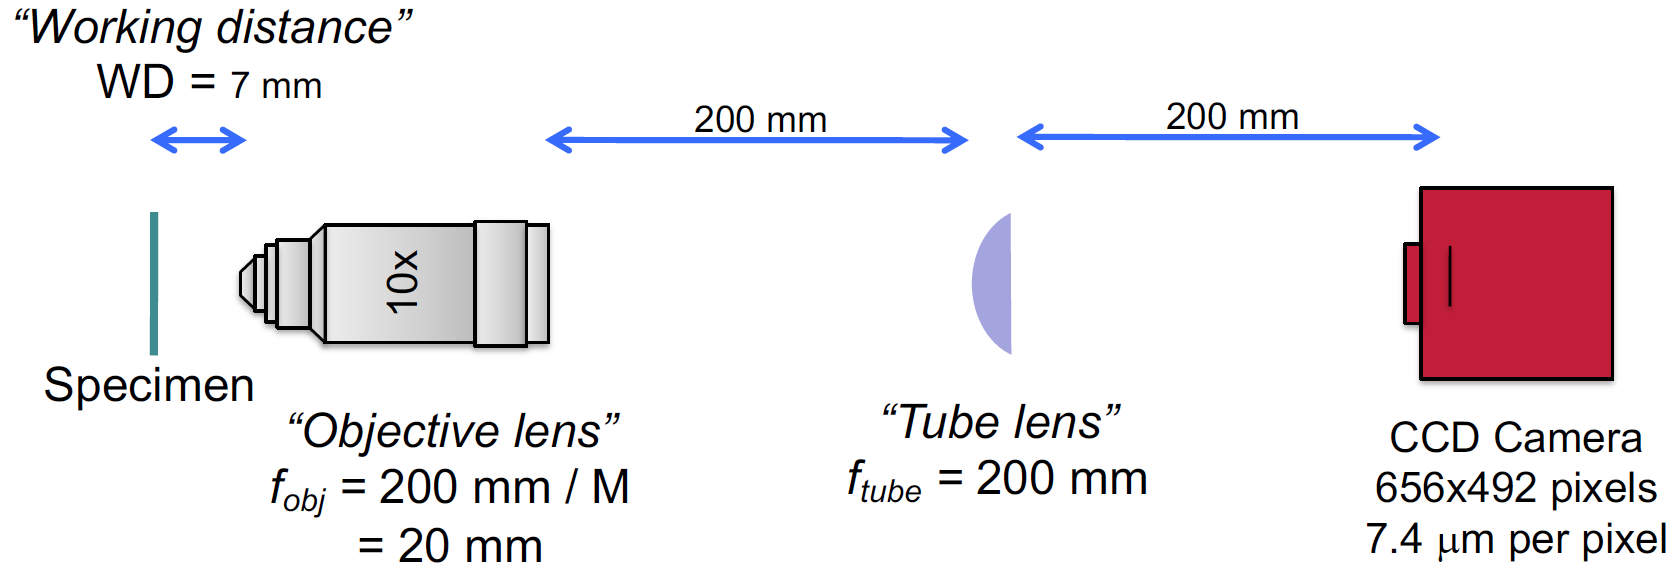
\includegraphics[scale=0.2]{Images/simple_microscope.png} 
Preparing biological specimen for imaging: Refractive index matching liquid between the specimen and the lens
determines the efficiency of light collection from the specimen, hence
brightness and resolution.

\subsubsection{Lens limitations}.\\
\textbf{Spherical aberration:} lightrays will not focus on the same point along the horizontal axis\\
\textbf{Coma:} lightrays will not focus on the same point on the vertical axis\\
\textbf{Chromatic aberration:} Lens fails to focus all wavelengths on the same point can use different sheets of lenses to compensate for this)\\
\subsubsection{Resolution} \label{Resolution}.\\
When can two point sources imaged onto a screen be distinguished? Each point source gives an airy disk on the screen:
 $I(\theta) = I_0 \left ( \frac{2 J_1(kd \sin \theta)}{kd \sin \theta} \right )^2 $, that can be distinguished when the maximum of one is not closer than the first minimum of the other. Where $ I_{0}$ is the maximum intensity of the pattern at the Airy disc center, $ J_{1}$ is the Bessel function of the first kind of order one, $ k = {2 \pi}/{\lambda}$ is the wavenumber, d is the radius of the aperture, and $ \theta$  is the angle of observation.\\
The first zero occurs at:  $\sin \theta \approx 1.22\,{\frac {\lambda _0 }{d}}$ $\implies$ larger aperture, thinner PSF, better resolution.\\
\textbf{Resolution:} \eqbox{R \approx f \sin \theta = 1.22 \lambda _0 f /d=0.61 \lambda _0 n/NA} (Rayleigh Criterion, works only when imaging process is only limited by diffraction)\\
\textbf{Standart terminology:} \emph{Numerical Aperture (NA): } measure of light gathering capacity. \eqbox{NA=n \sin \theta = n d/(2f)} with n the index of refraction\\
can't use to small wavelengths to not damage the biological specimen\\
\subsection{Illumination of sample}
Don't want to be blinded by the light that illuminates the sample
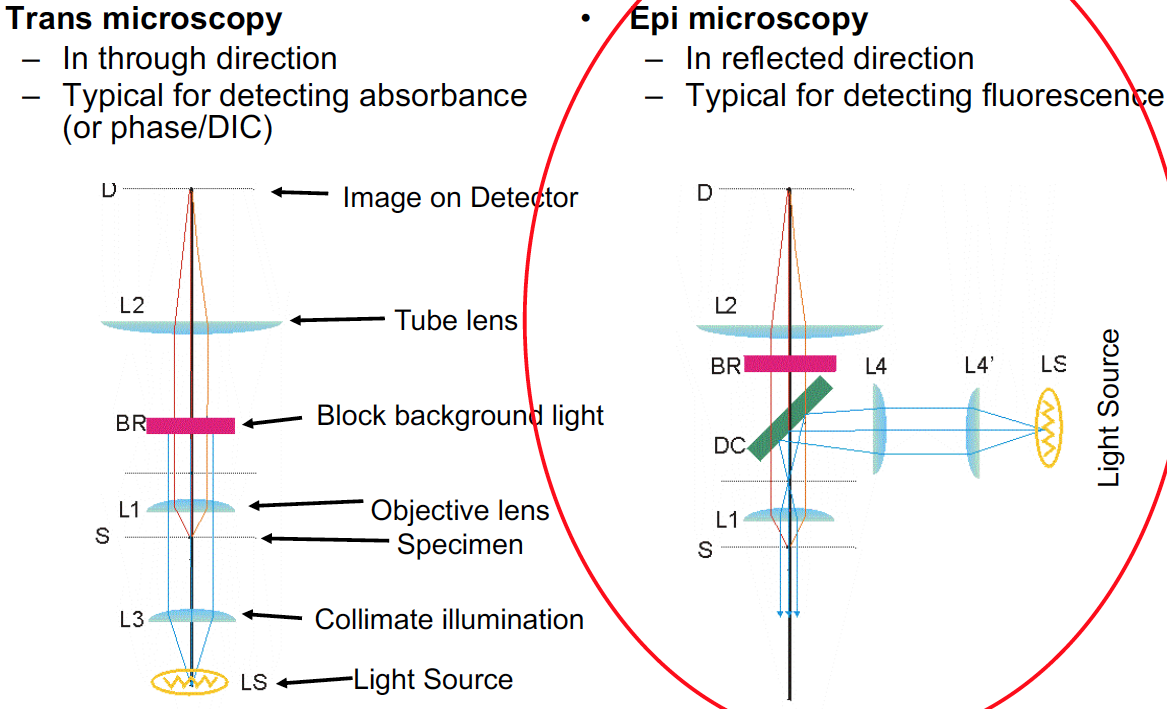
\includegraphics[scale=0.2]{Images/illumination_of_sample.png} blue lines = illumination light, orange lines = detected light\\
As we don't want our light to be focused on one point by the lens, we focus it at the objective back focal plane, so that it will then be evenly distributed on the sample (the objective lens will make the meams parallel). We also put a beam expander first.\\
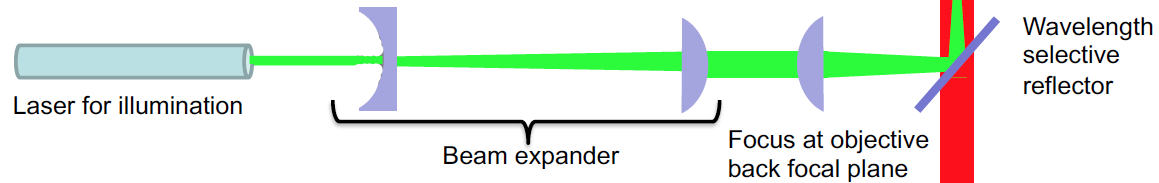
\includegraphics[scale=0.2]{Images/lightbeam_adaptations.png}
\subsection{White-light Microscopy}
Measures variations in refractive index, absorption, polarization and light-scattering. 
\textbf{Problems:} - Not specific enough to distinguish different types of molecules\\
- Not sensitive enough to detect single or even few molecules\\
- Cannot resolve objects much beyond the diffraction limit of light
\subsection{Fluorescence Microscopy}
\textbf{Fluorescence:} Photon absorption $\rightarrow$ electron excitation $\rightarrow$ electron loses some energy to nucleus vibrations $\rightarrow$ photon emission with less energy (gives a way to distinguish the illumination light to the reflected light)\\
It is best to illuminate the sample in it's peak absorption spectrum (PAS) and to capture in its peak emission spectrum (PES). The lamp light is first filtered by an "heat filter", which removes high $\lambda$. Above the sample is a filter which reflects PAS into the sample and let's the PES coming from the sample through.\\
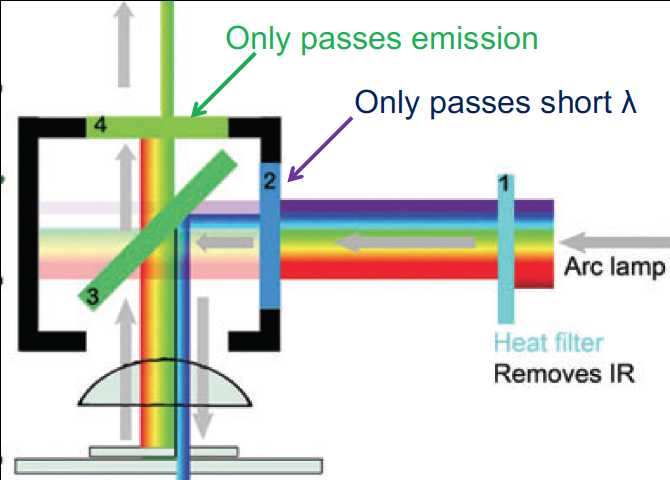
\includegraphics[scale=0.2]{Images/epi_setup.png}
The filters work with destructive interference and not with absorption.\\
\textbf{Ideal lightsource:} - Monochromatic (to excite the specimen at its peak absorption wavelength))\\
- High spectral radiance (for sufficient light intensity at particular wavelength)\\
- Low divergence - unidirectional (for tight focusing, or uniform illumination)\\
$\implies$ \textbf{Laser}
\section{Mechanical Sensors}	
\subsection{Surface Stress change detection}
Molecules on top of a slice will apply mechanical stress to the surface and bend it. When shinig light on it, the change in angle of the reflected beam can be measured to measure the stress. Problem is non-specific binding. Could still be used for scent detection, as there is not much NSB in air.\\
\subsubsection{Stress $\sigma \ [kg\cdot m^{-1}\cdot s^{-2}]$}
.\\
\textbf{Elastic media}: $\sigma =\frac{F}{A}= \mu \frac{\partial u}{\partial z}$, $\mu$ being the elasticity and u the displacement\\
\textbf{Viscous media:}	$\sigma =\frac{F}{A}= \eta \frac{\partial}{\partial z}(\frac{\partial u}{\partial t})$, $\eta$ being the viscosity\\
\textbf{Viscoelastic media:} $\sigma =\frac{F}{A}= \mu \frac{\partial u}{\partial z}+\eta \frac{\partial}{\partial z}(\frac{\partial u}{\partial t})$
\subsubsection{Equation of motion}.\\
			\begin{wrapfigure}{r}{0.4\linewidth}
			\vspace{-10mm}
								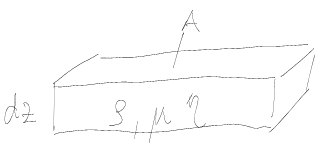
\includegraphics[width = 0.9\linewidth]{Images/equation_motion.png}
				\end{wrapfigure}
			$u=u(z,t)$;\\ $F=ma=m\cdot \frac{d^2u}{dt^2} \implies$\\
				\eqbox{\rho\frac{\partial^2u}{\partial t^2}=\frac{\partial}{\partial z}\Big(\mu\frac{\partial u}{\partial z}+\eta\frac{\partial}{\partial z}\frac{\partial u}{\partial t}\Big)}


			$\rho$=density\\
			$\mu$=elastic modulus\\
			$\eta$=viscosity\\
$u=u(z,t)$; $F=ma=m\cdot \frac{d^2u}{dt^2}$
\\ with $\rho$ being the density, $\tilde \mu=\mu +i \omega \eta $\\
harmonic solution: $u(z,t)=\tilde u (z)\cdot  e^{i \omega t}$ $\implies -\omega ^2 \rho = \tilde \mu k^2$\\
\textbf{Elastic media:} $\tilde \mu= \mu \implies k=\pm i\omega \sqrt{\frac{\rho}{\mu}}$\\
\textbf{Viscous media:} $\tilde \mu= i\omega \eta \implies k=\pm (i+1) \sqrt{\frac{\omega \rho}{2 \eta}}$\\
\emph{Solution to (1):} $\tilde u (z)=u_1 e^{kz}+u_2 e^{-kz}$\\
\textbf{Crystal of thickness l in vacuum:} $\omega _n=n \underbrace{\frac{\pi}{l}\sqrt{\frac{\mu}{\rho}}}_{\omega _0}$, $n=0,1,2,..$\\
\textbf{In water:} $\omega _n =n\cdot \omega _0+\Delta \omega _n$, $\Delta \omega _n = -\sqrt{n}\cdot \sqrt{\frac{\rho _w \cdot \eta _w \cdot \omega _0}{2}}\cdot \frac{1}{l\cdot \rho _q}$
\subsection{Cantilever based sensing}
			\begin{wrapfigure}[3]{r}{0.4\linewidth}
			\vspace{-7mm}
			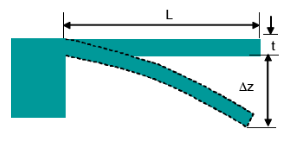
\includegraphics[width=0.9\linewidth]{Images/cantilever.png}
			\end{wrapfigure}
			$\Delta z=4\Big(\frac{L}{t}\Big)^2\frac{(1-v)}{E}(\Delta\sigma_1-\Delta\sigma_2)$\\
			E=Young's modulus\\
			v=poison's ratio\\
			$\Delta\sigma_1$=change in surface stress on top surface\\
			$\Delta\sigma_2$=change in surface stress on bottom surface\\
\subsection{Elastic plate in water}
	\begin{wrapfigure}[3]{r}{0.4\linewidth}
			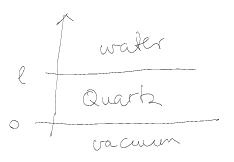
\includegraphics[width = 0.9\linewidth]{Images/plate.png}
		\end{wrapfigure}
		$\xi=e^{i\omega t}(\xi_1e^{kwz}+\xi_2e^{-kwz})$\\
		$u=e^{i\omega t}(u_1e^{kqz}+u_2e^{-kqz})$\\
		Boundary conditions:\\
		\boxed{
		\begin{aligned}
		& \frac{\partial u}{\partial t}\Big|_{z=0}=0\\
		& u(l)=\xi(l)\\
		& \tilde{\mu}_Q\frac{\partial u}{\partial z}\Big|_{z=l}=\tilde{\mu}_w\frac{\partial \xi}{\partial z}\Big|_{z=l}\\
		& \lim_{z\to\infty}=0\\
\end{aligned}	}		
\subsection{Quartz Crystal Microbalance}
\textbf{Piezoelectric effect:} Piezoelectricity is the electric charge that accumulates in certain solid materials (such as crystals, certain ceramics, and biological matter such as bone, DNA and various proteins) in response to applied mechanical stress.\\
Can use this effect to make the crystal resonate at resonance frequency \eqbox{f=\frac{n\cdot v}{\lambda}=\frac{n\cdot v}{2t}}.\\
 If a mass is added, the oscillation slows down: $\Delta m=Const\cdot \Delta f$
 Measure the frequency decay of the oscillation and the dissipation: $D=\frac{1}{\pi f \tau}$ ceveral times to get viscosity, elasticity, density and thickness of adsorbed layer.\\
 \textbf{Adsorption of rigid film in vacuum:} film: $\rho _f,\ d_f$; $\Delta f \propto \Delta m=\rho _f \cdot d_f$; $\Delta D = 0$\\
 \textbf{One side in an aqueous solution:} Fluid: $\rho _l,\ \eta_l$; $\Delta f,\ \Delta D \propto \sqrt{\rho _l\cdot \eta_l}$\\
 \textbf{Sauerbrey Model:} \\\eqbox{\Delta m= \frac{C}{n}\cdot \Delta f} with C: sensitivity factor, $n=0,1,2,..$ and $\Delta m= \rho \cdot h$ (for C $[\frac{ng}{Hz\cdot cm^2}]$, might need to multiply both $\Delta m$ and C by the area to get the right units/ the area should not appear in the end result)\\
  Is an approx. for thin adlayers
  \textbf{Sauerbrey equation}\\
			\eqbox{\Delta f=-\frac{2f_0^2}{A\sqrt{\rho_q\mu_q}}\Delta m},\enspace
			\\$f_0$=resonant frequency(Hz),\enspace
			$\Delta f$=Frequency change(Hz),\enspace
			$\Delta m$=mass change(g),\enspace
			$A$=Area between electrodes,\enspace
			$\rho_q$=density of quartz(=$2.648g/cm^3$),\enspace
			$\mu_q$=shear modulus of quartz(=$2.947\cdot10^{11}\frac{g}{cm\cdot s^2}$)
 \subsection{Strain gauge transducers}
 Measure change in resistance to measure strain:\\
 \grey{$\frac{\Delta R}{R}=K \frac{\Delta l}{l}=K \epsilon$}; $\epsilon:$ strain, $K$: Gauge factor ($\approx 2$), R: resistance\\
 Measure change in resistance on nanowires to measure strain: when nano-wire conductor gets elongated, some will lose touch and thus the resistance will go up, can attain extremely high gauge factors by controlling the contact resistance
 \subsubsection{Capacitive strain sensor }.\\
  $C=\epsilon _0 \cdot \epsilon _r \cdot \frac{A}{d}$ $\rightarrow$ change in capacitance will change the resonance frequency of RLC circuit $\omega _0= \frac{1}{\sqrt{LC}}$.\\
  Used to wirelessely control the bladder volume.\\
 \textbf{RLC circuit:} $V_L =L\cdot \frac{dI_{L}}{dt}$ $I_C=C\cdot \frac{dV_C}{dt}$
 \section{Fluorescent Probes}
 Use $\lambda = 510$nm for GFP markers.	
 \textbf{Photobleaching:} the photochemical alteration of a fluorophore molecule such that it permanently is unable to fluoresce. Increasing light intensity increases photobleaching (molecules have a limit to how much they can emit). \\
Photon Absorption $\rightarrow$ Electron Excitation $\rightarrow$ Electron Relaxation by excitation of nuclear vibrations $\rightarrow$ Photon Emission OR
Vibrational relaxation to ground state OR
Chemical Reaction (Photobleaching)\\
\textbf{Quantum Yield/efficiency:} \eqbox{\frac{\Gamma}{\Gamma + k +K_b}\sim 0-98\%}\\
\textbf{Fluorescence lifetime:} \eqbox{\tau = \frac{1}{\Gamma + k + K_b} \sim 1ns}\\
with $\Gamma$: radiative decay rate, k: non-radiative decay rate, $K_b$: photobleaching rate\\
fluorescence decay: $\frac{dN_e}{dt}=-(\frac{1}{\tau_1}+\frac{1}{\tau_2}+...)N_e $
	$\implies F=F_0e^{-\sum t/\tau_i}$
	$N_e$=\# of molecules in excited state\\
	$F$=fluorescence intensity ($N_e \propto F$)\\
\textbf{Measurement of decay}
		\begin{itemize}
			\item Pulsed illumination(time domain):\\
			after population of fluorophores is excited by delta pulse of light, the fluorescence 
			decay curve can be recorded by time-correlated single-photon counting (TCSPC)
			\item Phase modulation(frequency domain):\\
			the fluorescence gets $i)$ demodulated and $ii)$phase shifted by light source that is 
			modulated at high frequencies. From the two quantities $i)$ and $ii)$ the decay 
			time can be reconstructed.   
		\end{itemize}

\subsection{Fluorescence lifetime imaging} 
Decay of number of molecules in excited state: $\frac{dN_e}{dt}=-(k+\Gamma)N_e$\\
$N_e$: number of molecules in excited state\\
Decay in fluorescent emission intensity: $F=F_0e^{-(k+\Gamma)t}=F_0e^{-t/\tau}$\\
F and $F_0$ are the instantaneous and initial fluorescence intensity.\\
\emph{Fluorescence emission is characterized by exponential decay}.\\
\subsection{Förster resonance energy transfer (FRET)}
Excited molecule can transfer its energy to nearby (few nanometers) molecules. The emission is then going to be at the emission wavelength of the neighbour. $\rightarrow$ permits to measure if there is receptor/ligand interaction.\\
\begin{wrapfigure}[3]{r}{0.4\linewidth}
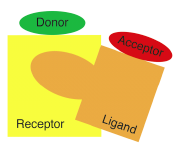
\includegraphics[scale=0.4]{Images/FRET.png}
\end{wrapfigure}
FRET is a dipol-dipole interaction and is very sensitive to r ($r^{-6}$)\\
\textbf{Efficiency of FRET:} \\\eqbox{E=\frac{R_0^6}{R_0^6 + r^6}=1-\frac{\tau _{DA}}{\tau _D}=1-\frac{I_{DA}}{I_D}}\\
DA/D: Donor with/without acceptor A, \\$\frac{\tau _{DA}}{\tau _D}$: Lifetime/Intensity of donor emission with/without acceptor, \\
 $I_{DA}/I_D$=ratio of the Intensities of donor emission with and without acceptor A
\\\textbf{Förster ditance:} $R_0=40$ to 70 \si{\angstrom} when efficiency of energy transfer is 50\%\\
\emph{Smaller distance $\rightarrow$ Reduced donor lifetime and donor emission intensity but higher acceptor emission intensity}\\
\emph{Larger distance $\rightarrow$ Low FRET, High fluorescence intensity, High average donor lifetime}\\
- Lightsource should excite donor but not acceptor -no overlap\\
- Need spectral overlap with donor emission and acceptor excitation spectrum for efficient energy transfer\\
\textbf{Photobleaching FRET:} (photobleaching: a fluorescent molecule can emit a limited number of photons by excitation befor it irreversibly converts to a non-fluorescent molecule):\\
\textbf{Sensitized emission:}
conclude FRET efficiency by measuring acceptor emission intensity. When donor and acceptor get
closer $\Rightarrow$ acceptor emission increases


\subsection{Calcium Imaging}
Calcium regulates cellular processes such as cell
division, muscle contraction, fertilization, blood
clotting, and synaptic transmission/plasticity $\rightarrow$ measure calcium to measure acitivity\\
\textbf{Idea:} Design molecules with optical properties that change upon calcium binding.\\
\textbf{Single wavelength measurements: }\\
.\\
$K_d=\frac{[Ca^{2+}]_i\cdot [Unbound\ dye \sim F_{max}-F]}{[Ca^{2+}-bound\ dye \sim F-F_{min}]}$\\
$\implies [Ca^{2+}]_i =K_d\frac{F-F_{min}}{F_{max}-F}$ with $K_d$: dissociation constant of the indicator, $F_{min}$: fluorescence at zero $Ca^{2+}$ concentration, $F_{max}$: fluorescence at saturating $Ca^{2+}$ levels. \emph{Problem:} need to know the dye concentration\\
\textbf{Dual-wavelength excitation measurements: } Do two measurements of fluorescence $F_1$ and $F_2$ which are depending on excitation wavelength. $R=\frac{F_1}{F_2}$\\
$[Ca^{2+}]=K_{eff} \frac{R-R_{min}}{R_{max}-R}$ with $R_{min}$: ratio in $Ca^{2+}$ free solution, $R_{max}$: ratio at $Ca^{2+}$ saturating levels, $K{eff}$: effective binding constant
\subsubsection{Principles of different calcium indicators}.\\
- The binding of  $Ca^{2+}$ leads to a change in fluorescence intensity but not
wavelength change (fluo-4, rhod-2, calcium green)\\
- The binding of $Ca^{2+}$ results in a shift in excitation and sometimes emission
peaks – ratiometric indicators (fura-2, quin-2, indo-1)\\
- The binding of $Ca^{2+}$ results in changes in fluorescent resonance energy
transfer (FRET e.g. chameleons)
- The binding of $Ca^{2+}$ leads to a change in fluorescence life time (FLIM, e.g.
indo-1)
\subsubsection{Delivery of Calcium Indicators to Cells}.\\
Loading cells using acetoxymethyl (AM) esters of $Ca^{2+}$ indicators: AM will neutralise the charge of indicator, which will permit it to cross cell membrane. Inside the cell the indicator will get charged (thus becomes trapped in cell) and becomes fluorescent. Cautions: too high concentration of indicator can alter $[Ca^{2+}]$ and generate toxic byproducts.\\
A dye with too high $Ca^{2+}$ affinity: very sensitive, but very slow recovery\\
A dye with too low $Ca^{2+}$ affinity: very insensitive, but very fast recovery
\section{Signal and Noise}
\textbf{Technical noise}: due to detector imperfections -can be avoided by good design\\
\textbf{Sum of all noises:} $\langle I_{noise}^2 \rangle =\langle I_s^2\rangle + \langle I_D^2 \rangle + \langle I_J^2 \rangle$\\
\textbf{Total Noise:} $N_{noise}  = N_s+N_D+N_I$\\
	SNR(\textbf{S}ignal to \textbf{N}oise \textbf{R}atio): Signal power/Noise power\\
	NEP(\textbf{N}oise \textbf{E}quivalent \textbf{P}ower): Signal power at which SNR=1\\
\subsection{Shot Noise}
\textbf{Shot Noise ($N_s$)}: Shot noise exists because phenomena such as light and electric current consist of the movement of discrete 'packets'. It is is temperature and frequency independent. Statistical fluctuation of uncorrelated random events obey \textbf{Poisson statistics}: $P(n|\bar{n})=e^{-n}\frac{\bar{n}^n}{n!}$, \eqbox{\sigma _n = \sqrt{\bar{n}}=\sqrt{<signal>}}\\
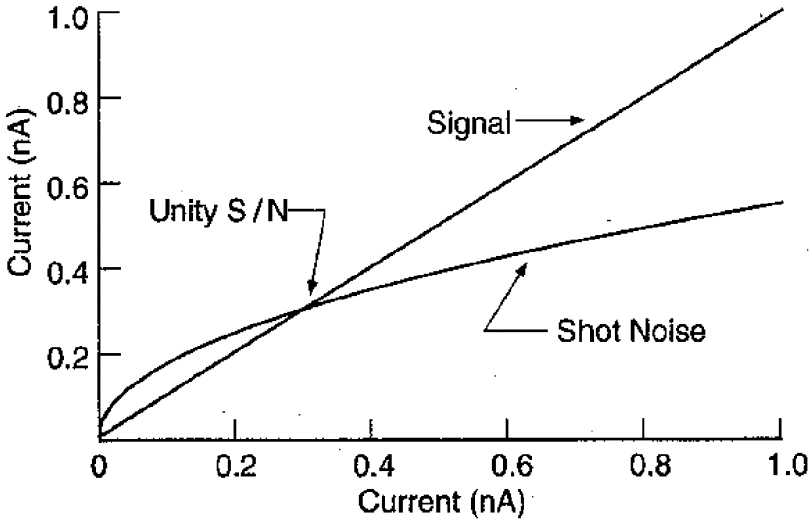
\includegraphics[width = 0.5\linewidth]{Images/shot_noise.png}\\
$<I_{noise}^2>=(\eta q/\Delta t))<I_{signal}>$ \\
$\implies$ $<I_{noise}> \propto \sqrt{<I_{signal}>} $, with $\eta$: quantum efficiency of detector, $\bar{n}$: \# photons, q: el. charge	\\
\textbf{Signal Power:} $S=<I_{signal}^2>R$\\
\textbf{Noise Power:} $N=<I_{noise}^2>R$	\\
\textbf{Noise equivalent power (NEP):} Signal power at which SNR =1\\
\eqbox{N_s=<I_{noise}^2>R=2R\eta q B<I_{signal}>}, with $2B\approx 1/\Delta t$: bw.\\
\textbf{Responsivity:} \eqbox{<I>/P=\eta q \lambda/(hc)}\\
\textbf{SNR:} \grey{$\frac{P \lambda}{2hcB}=\bar{n}$}\\
\eqbox{{<}I_{signal}{>}=\eta q \bar{n} /\Delta t} \eqbox{{<}I_{noise}{>}=\eta q \sqrt{\bar{n}}/\Delta t}
	\eqbox{{<}I_{noise}^2{>}=(\eta q /\Delta t){<}I_{signal}{>}} \\
	\eqbox{\Rightarrow {<}I_{noise}{>} {\propto} \sqrt{{<}I_{signal}{>}}}\\
	\eqbox{SNR_{power}=\frac{P \lambda}{2 h c B}=\bar{n}}\\
$\bar{n}$ = mean number of detected photons = $\frac{1}{M}\sum\limits_i^M n_i$\\
					M=\#of measurements\\
					Variance $\sigma_n^2=\frac{1}{M}\sum\limits_i^M (n_i-\bar{n})^2$,\enspace\enspace
					$\sigma_n=\sqrt{\bar{n}}$\\



\subsection{Dark current Noise}
Thermal effect results in some probability of spontaneous production of free electrons. This effect is measured by the dark current amplitude of the device:$<I_d>$. $N_d$ also obeys Poisson statistics: \grey{$N_d=2R\eta q B<I_d>$}

\subsection{Jonson Noise}
Johnson noise ($N_j$) originates from the temperature dependent fluctuation in the load resistance R of the detection circuit.\\
\eqbox{I_J \propto \sqrt{\frac{kTB}{R}}}\eqbox{N_J{\propto}I_J^2R}	\\
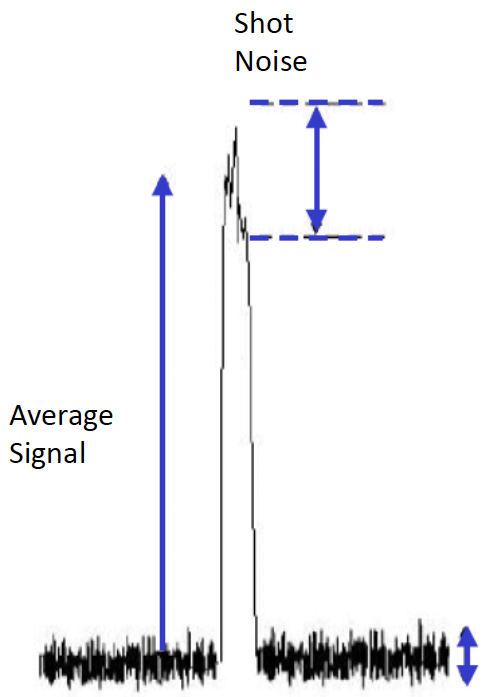
\includegraphics[scale=0.1]{Images/noise.png} shot noise dominates other noise at for large signal
\section{Optical Detectors}
- \textbf{Quantum Efficiency (QE):} The probability of generating a photoelectron from
an incident photon\\
- \textbf{Internal Amplification:} The amplification ratio for converting a photoelectron
into an output current\\
- \textbf{Dynamic Range:} What is the largest and the lowest signal that can be
measured linearly\\
- \textbf{Response Speed:} The time difference and spread between an incoming
photon and the output current burst\\
- \textbf{Geometric form factor:} Size and shape of the active area and the detector\\
- \textbf{Noise:} Shot noise vs. read-out noise dominated\\
\eqbox{SNR= \dfrac{<signal>}{\sigma _{signal}}= \dfrac{QE\cdot N_{\gamma}}{\sqrt{\sigma_{D}^2+\sigma_{R}^2+\sigma_{S}^2}}}, QE: quantum efficiency,\\ $N_{\gamma}$: \# detected photons
\subsection{Photoelectric effect}
$hf=\phi + E_k$: incident photon energy = binding energy ($\phi$ is the work function) + kinetic energy of ejected electrons\\
- The kinetic energy of emitted electron depends only on the color (wavelength) of the photon
but not light intensity (number of photons)\\
- The number of electrons ejected is proportional to the intensity (number of photons)
\begin{wrapfigure}[9]{r}{0.1\textwidth}
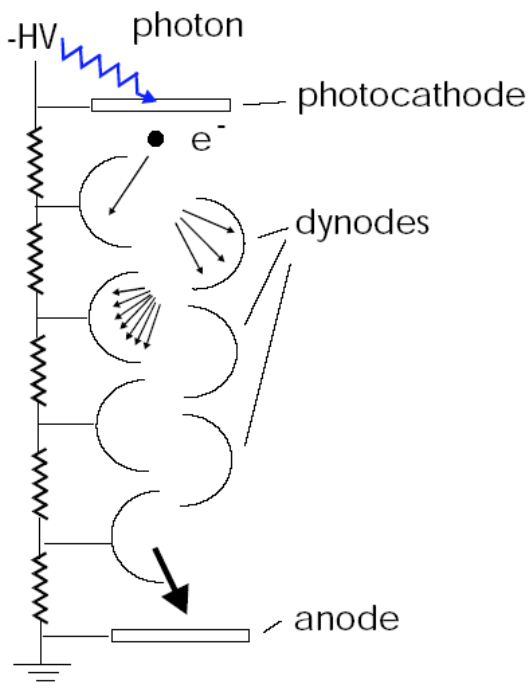
\includegraphics[width=0.1\textwidth]{Images/photomultiplier_tube.png}
\end{wrapfigure}

\subsection{Photomultiplier tube}
$I=\alpha\cdot (S\cdot E_{\gamma}\cdot n/\Delta t)$ with S the \textbf{Cathode sensitivity} and $\alpha$ the \textbf{gain}. $E_{\gamma}=hc/\lambda= 4\cdot 10^{-19}J$
\subsection{Photovoltaic Effect}
Electron-hole pair generation in semiconductor by incident light $\rightarrow$ the quantum efficiency of detector $\eta$ is strongly wavelength dependent, because photons with energy less than Eg cannot generate conducting e-h pairs. The electrons are then moved via \textbf{CCD} (charge-coupled detectors -bucket arrays) or via CMOS to be analyzed. CMOS can be faster, but less uniform, noisier than CCDs.\\
\textbf{Readout Noise:} The noise that the camera’s amplifier circuit introduces (specified in spec sheets). It is a combination of Johnson Noises + Amplifier Technical Noise. $N_{total}=N_{readout}+N_{dark}+N_{shot}$ $\rightarrow$ has high temperature dependency, can cool down to limit noise.\\
Can overcome readout noise with \emph{Electron-multiplication CCDs (EM-CCDs)}: amplify
electrons prior to amplifier circuit by impact ionization on the chip.\\
\subsection{Pixel size}
Separation of diffraction limited spots on CCD:\\
 $\Delta x \cdot (f_t/f_o)=0.61(\lambda/NA)\cdot M$ (magnification $M=f_t/f_o$) see \ref{Resolution}\\
\textbf{Maximum pixel size:} \eqbox{0.5\cdot \Delta x\cdot M=0.3\cdot (\lambda/NA)\cdot M} (Nyquist)\\
Too large pixels $\rightarrow$ cannot resolve the image\\
Too small pixels $\rightarrow$ too little signal/photon per pixel $\rightarrow$ readout circuit noise dominates\\
If CCD pixels are smaller than minimum pixel size OR if there is too little signal, then sum the neighboring pixels (\emph{pixel binning}) to increase signal.
\subsubsection{How to choose a camera with the right number of pixels?}.\\
- First make sure \textbf{FOV} of objective (specified by manufacturer) is large enough for what you want to see. FOV= magnification$\cdot $ NA\\
- Choose a region of interest (\textbf{ROI}) size within FOV of lens: Specimen within ROI is magnified M times: 250\si{\micro\meter} ROI w/ M=40 $\rightarrow$ you need 10 mm CCD size.\\
- Number of pixels: [CCD Area] / [Pixel size matching diffraction limit]\\
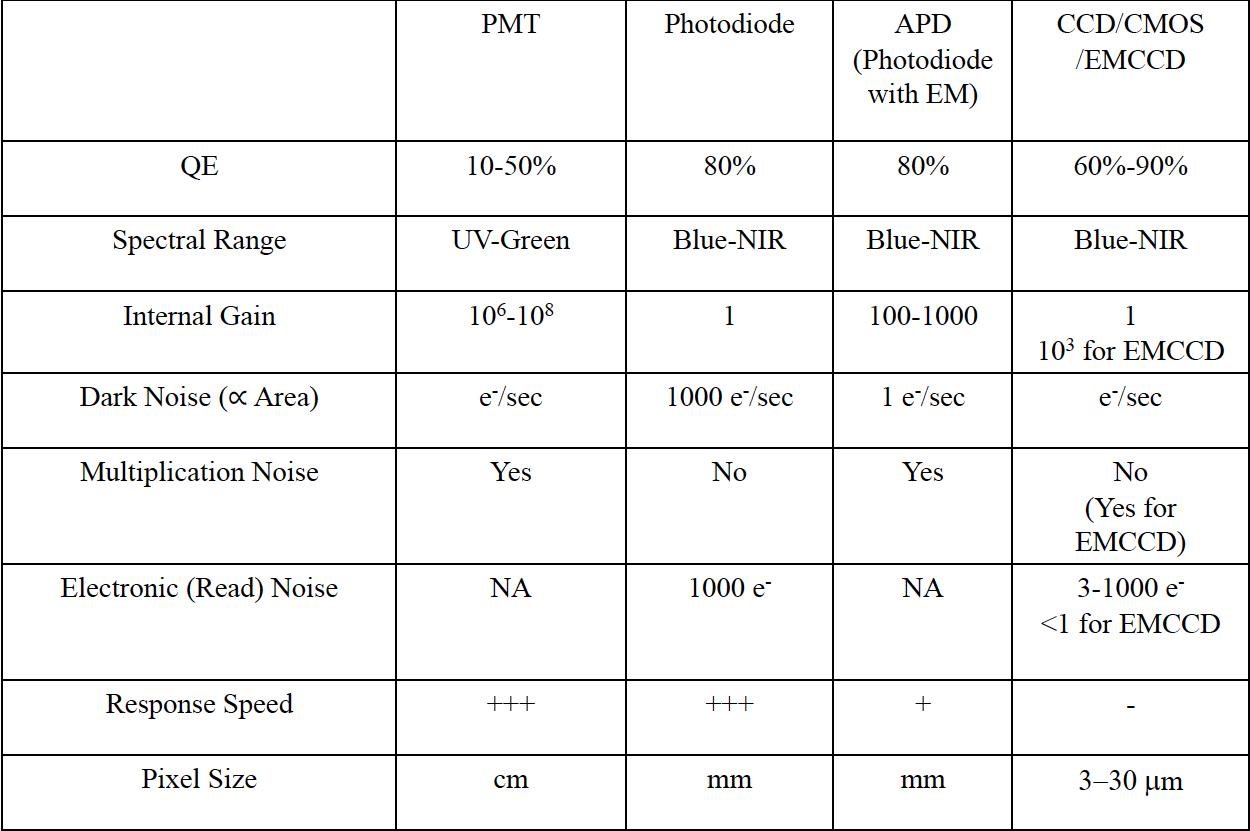
\includegraphics[width = \linewidth]{Images/comparison_detectors.png}
\\



\section{Scanning Microscopy}
Problems: - out of focus absorption $\rightarrow$ bleaching \\
- scattering of light rays in sample $\rightarrow$ SNR$\downarrow$
\subsection{Confocal Microscope}
\begin{wrapfigure}[19]{l}{0.23\textwidth}
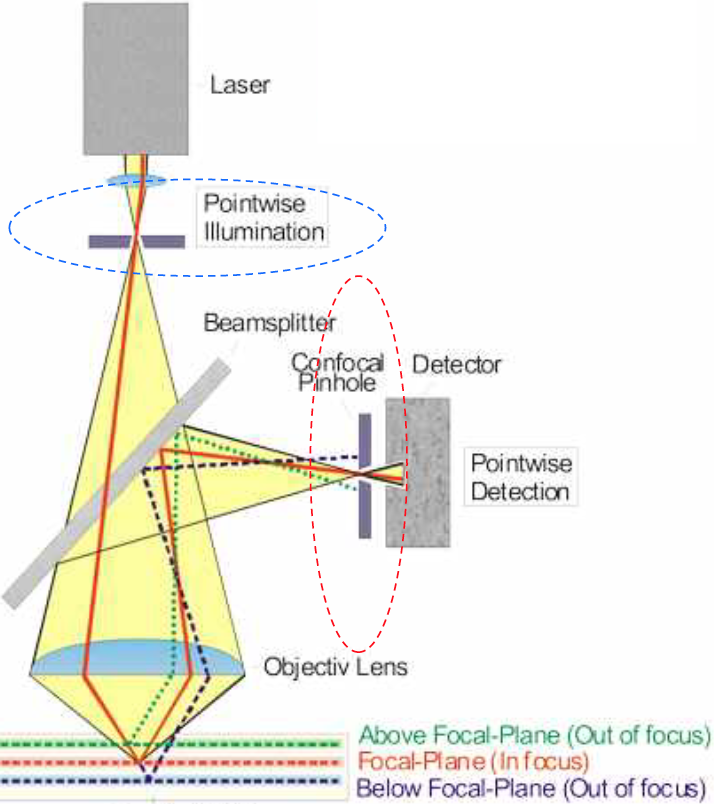
\includegraphics[width = \linewidth]{Images/confocal_microscope.png}
\end{wrapfigure}
- Constrain/focus the illumination to a small spot\\
- Rejects other fluorophores at different locations and scattered fluorescence\\
- Collect all the light onto a single detector i.e. photomultiplier tube (more efficient than CCD)\\
$\rightarrow$ results in flattening of sinc ripples in PSF and narrows FWHM\\
 Smaller pinhole: Higher xy and depth resolution BUT Less signal $\rightarrow$ Slower imaging\\
 .\\
Smallest pinhole size should be proportional to the resolution of the rest of the optical system: \eqbox{\text{Pinhole size} \sim (0.61\cdot \lambda /NA)\cdot M)}\\
Faster scan: Less bleaching, observe fast physiology\\
Slower scan: Collect more photons per point (higher SNR, higher resolution/contrast) but increased bleaching\\
Image one point of sample $\rightarrow$ need to scan with the lasers to get full image. Direct laser with mirrors for x-y dimensions and move lens for $\vec{z}$\\
\textbf{Upgrade:} Confocal Nipkow spinning-disk: 
- Multiple laser points simultaneously illuminating the sample: Array of confocals.\\
- Spin the disc quickly to collect data from all the points on sample very fast
- Limitation: needs CCD, which are less efficient than PMT's.\\
\textbf{Problems:} Still has out of focus absorption and scattering for illumination and emission + highly inefficient.\\
\textbf{Solution:} Two-photon excitation: if material interacts at freq. f, send light at f/2 that meets in focal point. For each excitation, two photons of f/2 are absorbed. As only light with freq. f interacts with the material, there is no scattering and no out of focus absorption.\\
 $\rightarrow$ less photobleaching\\
 $\rightarrow$ no need for pinhole for lightsource nor for detector (one knows exactly where the photons come from, so scattering is no issue)\\
 \textbf{Disadvantages:} Need special lasers with ultrashort-light pulse s.t. likelihood of two photons simultaneously hitting/exciting fluorophore is high.\\
 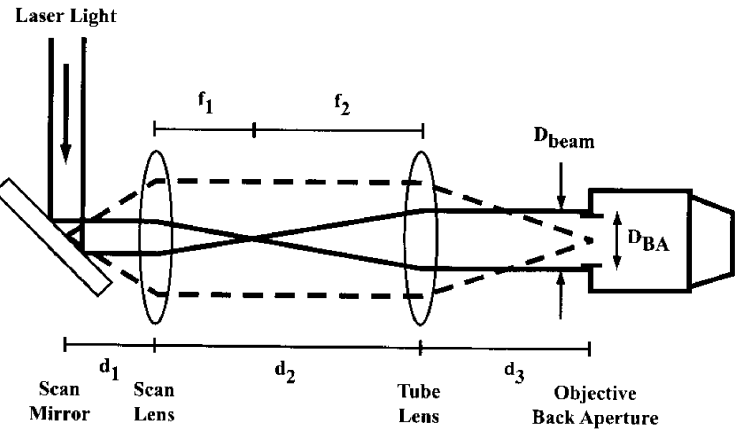
\includegraphics[scale=0.15]{Images/2ph_microscope.png}
$d_2=f_1+f_2$; $d_1=\frac{f_1^2}{f_2}+f_1-d_3(\frac{f_1}{f_2})^2$
\section{Optical Biosensors}
	\subsection{Formulas}

			\eqbox{c_0=\frac{1}{\sqrt{\epsilon_0\mu_0}}}
			\eqbox{\frac{2\pi}{\lambda_0}=k_0=\frac{\omega}{c_0}=\omega\sqrt{\epsilon_0\mu_0}}
			\eqbox{n_i=\frac{c_0}{c_i}=\sqrt{\epsilon_i\mu_i}}
			\eqbox{\frac{n_1}{n_2}=\frac{sin\theta_2}{sin\theta_1}}
			\eqbox{\theta_{crit}=arcsin(\frac{n_2}{n_1})}\\
			Maxwell equations:\\
			\begin{wrapfigure}{l}{0.2\linewidth}
			\vspace{-05mm}
			    \boxed{\begin{aligned}
				&\partial_t\vec{D}=\vec{\nabla}\times\vec{H}\\
				&\vec{\nabla}\cdot \vec{D}=0\\
				&\partial_t\vec{B}=-\vec{\nabla}\times\vec{E}\\
				&\vec{\nabla}\cdot\vec{B}=0
			\end{aligned}}	
			\end{wrapfigure}
					
			Assumptions:$\vec{D}=\epsilon\vec{E}$,\enspace
			$\vec{B}=\mu\vec{H}$,\enspace
			$\mu=1$\\
 \textbf{Ellipsometry: }Change in the phase and amplitude of the polarized light provides information about the thickness and
refractive index of the adsorbed protein layer.\\
\eqbox{\frac{R_p}{R_s}=tan\Psi e^{i\Delta}} R=reflection coefficient\\
\textbf{Optical Immuno Assay: } Optical film resonates with certain wavelengths, changes with thickness of film.
    \subsection{Surface Plasmon Resonance}
\begin{wrapfigure}[15]{l}{0.25\textwidth}
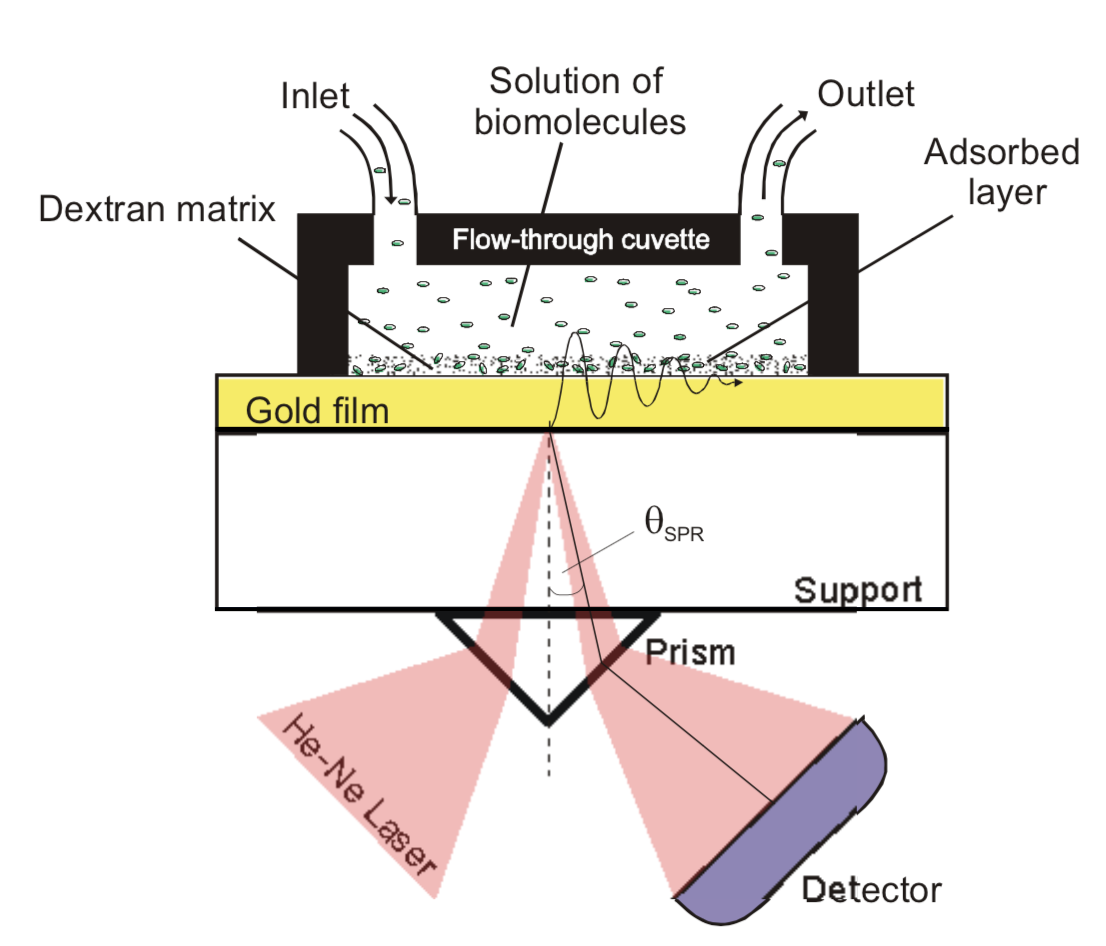
\includegraphics[width=\linewidth]{Images/surface_plasmon_resonance.png}
\end{wrapfigure}
\textbf{Evanescent Field: } $E(z)=E_0 e^{-z/d_p}$\\
Depth of penetration: $d_p = \frac{\lambda}{4\pi \sqrt{n_1 ^2 \sin ^2 \theta -n_2 ^2}}$\\
A resonant coupling between the light and the surface plasmons in the conducting film occurs at a specific angle.The reflected light will have a "shadow“ at the resonance angle. This angle is \textit{sensitive to the adsorption of proteins at the interface}. \\
.\\
Plasmons lose their energy if their momentum equals that of the incoming wave: $\beta = \frac{\omega}{c}\sqrt{\frac{\epsilon _m \epsilon _d}{\epsilon _m + \epsilon _d}}$\\
\textbf{Plasmonic hot spot: } Plasmons can also propagate on electron clouds inside a metal $\implies$ if particles close together, plasmons can interact contructively and change $\lambda$ of reflected light

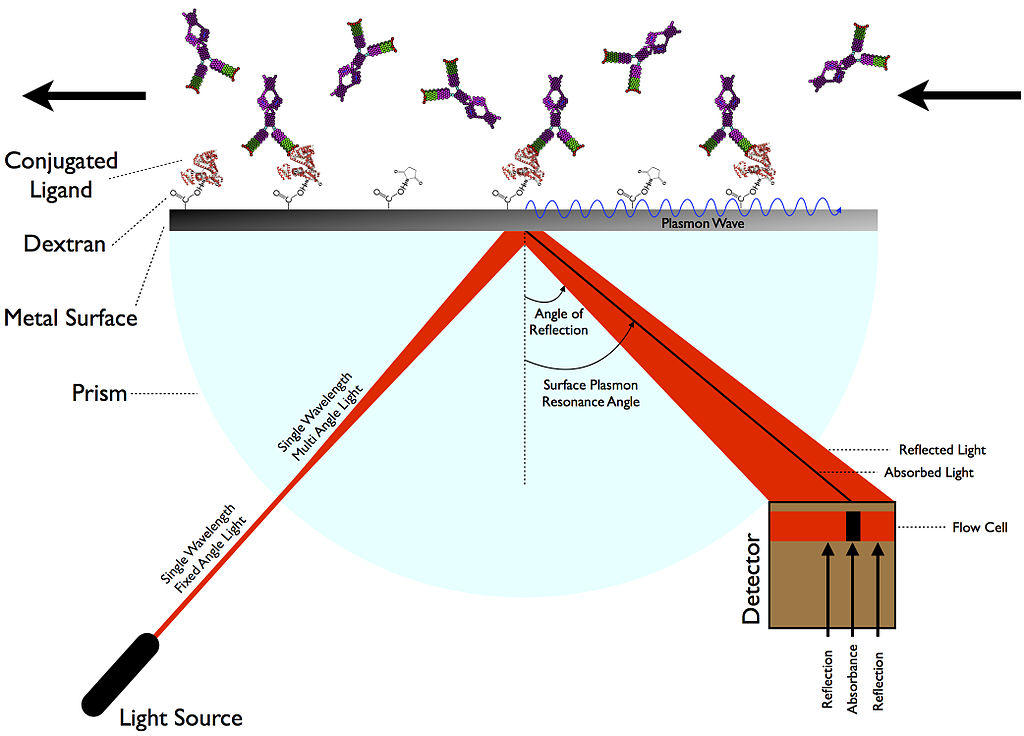
\includegraphics[width=0.5\linewidth]{Images/Surface_Plasmon_Resonance.jpg}

\textbf{Advantage:} label free, in situ,  imaging possibility(10$\mu m$ lateral resolution), $0.1ng/cm^2$ sensitivity\\
\textbf{Problems:} requires noble metal surface, measures only one parameter(calibration needed)
				
\textbf{Optical waveguide lightmode spectroscopy(OWLS):}\\
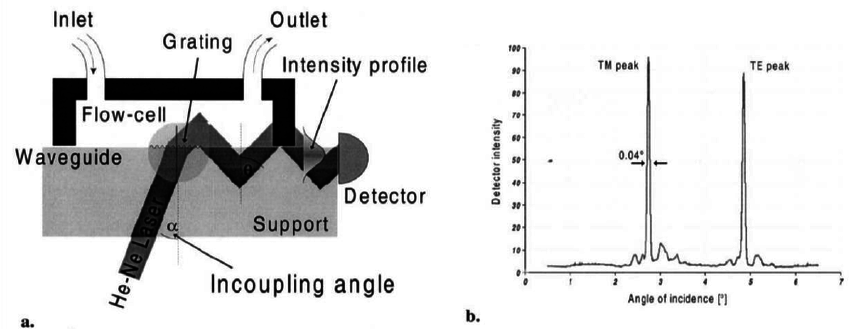
\includegraphics[width=\linewidth]{Images/OWLS.png}
\underline{Principle}: light is coupled into optical waveguide via optical grating
and intensity is measured as a function of the incident angle $\alpha$.
From the two peaks in the intensity spectrum(incoupling angles), the thickness and
refractive index of the adsorbed layer can be calculated.\\

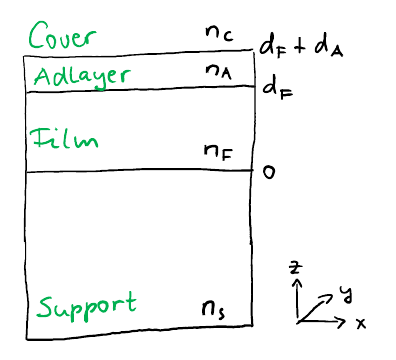
\includegraphics[scale=0.3]{Images/OWLS2.png}
$E_c e^{-ik_C(z-d_F-d_A)}$\\
$E_{A,1}e^{-ik_A(z-d_F)}{+}E_{A,2}e^{ik_A(z-d_F)}$\\
$E_{F,1}e^{-ik_Fz}{+}E_{F,2}e^{ik_Fz}$\\
$E_Se^{ik_Sz}$\\
\underline{Summary}: 
-label free,in situ 
-measures $d_A$,$n_A$ 
-sensitivity: $1ng/cm^2$ 
-requires waveguides 

    \section{Molecular Adsorption and Electron Transfer}
        \subsection{Schrödinger Equation}
        $\hbar = \frac{h}{2\pi}=1.055\cdot 10^{-34}\ Js$\\
        $\Psi(r,\theta, \phi)=R(r)\gamma(\theta,\phi)$\\
        Stationary: $\hat{H}\ket{\psi}=E\ket{\psi}$\\
        	time independent: $\hat{H}\ket{\psi}=i \hbar \frac{\partial \ket{\psi}}{\partial t}$\\
        Hamiltonian $H=$ kinetic energy + potential energy $= T+V=-\frac{\hbar ^2}{2m} \Delta ^2+V$\\
        One electron solution (Hydrogen Atom):\\
        $H=T_n + T_e+V{n-e}$ $\implies$ $-\frac{\hbar ^2}{2m}\Delta ^2 \Psi - \frac{Z e^2}{4 \pi \epsilon_0 r}\Psi=E\Psi$, $E=\frac{\hbar ^2 k^2}{2m}$\\
       
       
        
\begin{comment}

\subsection{Infinite quantum well}

\[
    V(x)= 
\begin{cases}
    0,      & \text{ if } 0<x<a\\
    \infty, &  x<0 \text{ or } x>a
\end{cases}
\]
\[  \Rightarrow \psi(x)= 0 \text{ if } x<0 \text{ or } x>a\]
Continuity Condition
\[ \psi(x)=\psi(a)=0\]
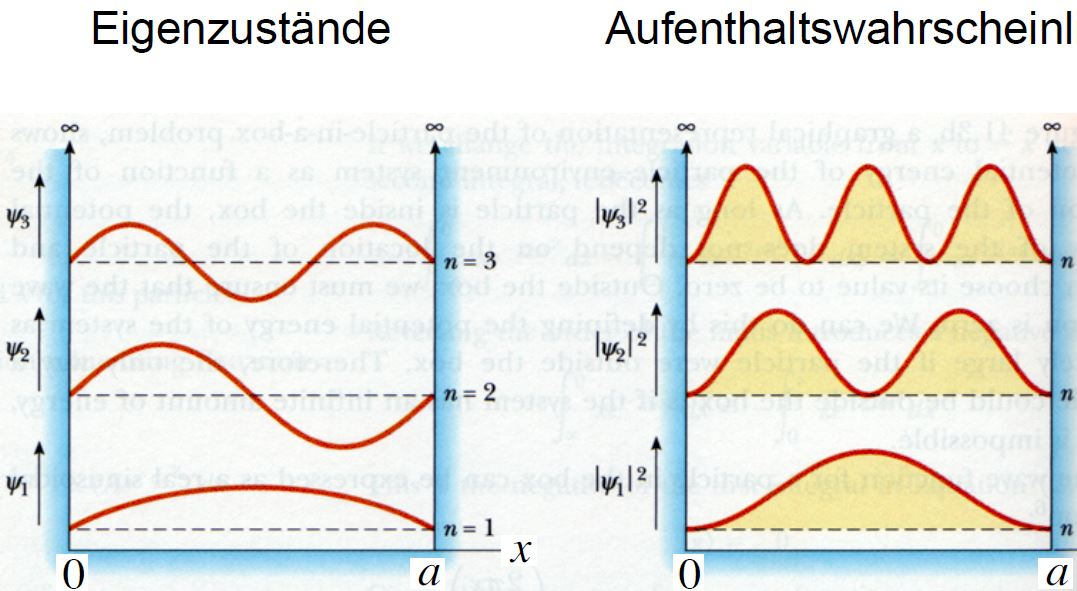
\includegraphics[width=0.3\columnwidth]{Something/Images/unendlich.JPG}

\begin{enumerate}
    \item General solution: \\
    $ \psi(x)= Ae^{ikx}+Be^{-ikx}=A'\sin(kx)+B'\cos(kx)$
    \item Continuity condition:\\
     $\psi(x=0) =0 \qquad  \Rightarrow A= -B $
    $ \Rightarrow \psi(x) = A[e^{ikx}-e^{-ikx}] =A\cdot 2i \cdot sin(ka) $
    $ \psi(x=a) =0 \Rightarrow k_n=\frac{\pi}{a}n \text{ wobei } n=1, 2, ...$
    \item Not trivial solution
    $  \Rightarrow \psi(x) = \text{const} \cdot sin(k_n\cdot x)$
    \item Normalization
    $
        \INT{-\infty}{\infty}{\vert\psi(x,t)\vert^2}{x} = \vert \text A \vert^2 \cdot \INT{0}{a}{sin^2 \left( \frac{n\pi}{a}x \right)}{x}= \vert A \vert^2\cdot\frac{a}{2} \stackrel{!}{=}1 
    $
    $ \Rightarrow A= \sqrt{\frac{2}{a}}$
\end{enumerate}

\textbf{Energy: }
$  E_n=E_{kin,n,}= \frac{p_n^2}{2m}=\frac{(\hbar k_n)^2}{2m}=\left(\frac{\hbar^2 \pi^2}{2ma^2}\right)n^2 $

\textbf{Nullpunktenergie/tiefst erreichbare Energie:}\\
$E_{n=1}\neq 0 !$ 

\textbf{Erwartungswert infinite quantum  well}\\
 $\Braket{x}= \frac{a}{2}$ unabhänging von der Zeit
\end{comment}


Linear combination of atomic orbitals molecular orbital: $\Phi _i= \sum_{k} C_{ij} \Psi{j}$\\
A= \# electrons in bonding MO\\
B= \# electrons in anti-bonding MO\\
\textbf{Bond Order: } $\frac{A-B}{2} (\neq 0$ for stability)\\
\begin{wrapfigure}[6]{l}{0.185\textwidth}
	\vspace{-15pt}
		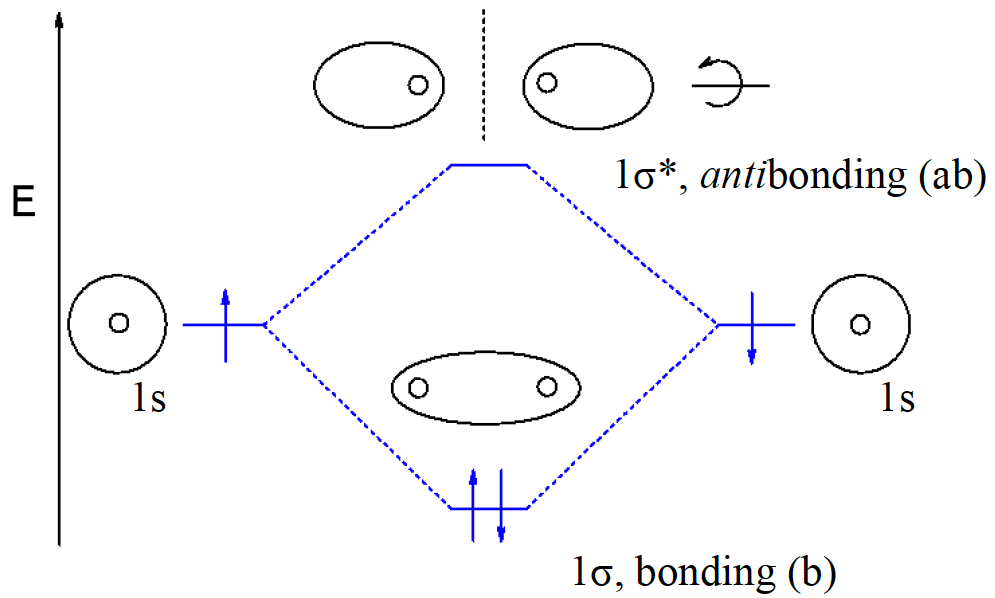
\includegraphics[width=0.9\linewidth]{Images/bonding_antibonding.png}\\
	\end{wrapfigure}

\textbf{HOMO:} Highest Occupied MO\\
\textbf{LUMO:} Lowest Unoccupied MO\\\\\\
\subsection{Formation of Crystal bands}
For each atom, 1 energy level: infinite Atoms $\rightarrow$ infinite energy levels\\
\textbf{Fermi-Dirac distribution: } $f(E)=\frac{1}{e^{(E-E_F)/(k_BT)}+1}$\\
\subsection{Adsorption}
\textbf{Physisorption: } depends on van der Waals interaction, process in which the electronic structure of the atom or molecule is barely perturbed upon adsorption.\\
\textbf{Chemisorption: } depends on overlapping integral: $S_{ij}=\int \Psi _{mol,i} \Psi _{substr,j}dxdydz$ $\implies$ charge transfer/sharing between surface and molecule\\
\textbf{Electrostatic Interaction: } $U_{coul}=\sum _{i\neq j} \frac{q_i q_j}{\epsilon _r \epsilon _0 |\vec{r_i}-\vec{r_j}|}$\\
\subsection{Electron transfer}
\textbf{Gibbs free energy: } thermodynamic potential that can be used to calculate the maximum of reversible work that may be performed by a thermodynamic system at a constant temperature and pressure \\
$G=U+p\cdot V-T\cdot S$, U: internal energy; P: pressure; V: volume; S: entropy\\	
G is minimized when the system is in chemical equilibrium @T=const. p=const.
\eqbox{\textbf{Reaction rate: }k\propto e^{-\frac{\Delta G}{RT}}}; $R=\frac{k_B}{N_A}=8.3\ J\cdot K^{-1}\cdot mol^{-1}$, with $\Delta G$: acitvation energy\\
\eqbox{\textbf{Rate of electron transfer: }k_{et}=K_{P,O}\cdot \nu _n \cdot \kappa _{el}\cdot e^{-\frac{\Delta G}{RT}}}\\
\textbf{number of occupied states: }$N_{occ}(E)=f(E) \cdot \rho (E)$, $\rho$: densitiy of states\\
In nanowires:  $k_{el}(x)=k_{el}^0\cdot e^{-\beta x}$ $\rightarrow$ exponential decay of the transmission coefficient with x

\section{Potentiometric Biosensors}

     \textbf{chemical potential: } 
     \\\eqbox{\mu _j=\Big(\frac{\partial U} {\partial N_i}\Big)_{S,V,N_{j\neq i}} =(\frac{\partial G}{\partial n_j})_{p,T,n'}}, with G the Gibbs free energy\\
    			$dG|_{p,T}=(\mu_B-\mu_A)d\xi$\\ 
     \textbf{Equilibrium} $\rightarrow$ $dG|_{p,T}=0 \implies$ \grey{$\mu _B=\mu _A$}\\
     \textbf{electrochemical potential: }$\bar{\mu _j}=\mu _0 +Z_jF \Delta \phi$ (for a metal, $\mu _0 = E_F$ at T=0K), $F=eN_a$ (Faraday constant)\\
     $\mu _{redox} = E'$ where $D_0(\lambda,E')=D_R(\lambda,E')$\\
     $\Delta \varphi = -\frac{\Delta _r G}{ZF}=C'+C_2\cdot \ln [ion]$; C',$C_2$ constants\\
     
     \eqbox{\textbf{Nernst Equation: }\Delta \varphi= \Delta \varphi _c ^0-\frac{RT}{nF}\cdot ln(Q) = C_1+C_2\ln(a_{ion})}, \\with $R=N_A k_B$, $Q=\frac{[Red]}{[Ox]}$\\
     
     
     \grey{General Nernst equation for $A\cdot ox +B\cdot X+z\cdot  e^- \underset{k_{ox}}{\stackrel{k_{red}}\rightleftharpoons} C\cdot  red+ D \cdot  Y$:}\\
     \eqbox{E=E^0 + \frac{R\cdot T\cdot 2.303}{F\cdot Z}\log (\frac{a_{ox}^A\cdot a_X^B}{a_{red}^C\cdot a_Y^D})} ($\ln (Q)=2.303\cdot  \log (Q)$)\\ 
      $a_{ion}=r_{ion}\cdot [ion]/1\frac{mol}{L}$ (activity coeff r often 1), $a_{gas} = p_{gas}/1.1013bar$, $a_{solid} =1$, \grey{$\frac{R\cdot T\cdot 2.303}{F}=0.059V$ at $ 25ºC$}\\
      Nernst for whole cell: $\Delta E= E_1-E_2= E_1^0-E_2^0+\frac{0.059V}{z}\cdot \log (\frac{Q_1}{Q_2})$ if $z_1=z_2$\\
     Reduction: gain of electron, Oxidation: loss of electron\\
     \emph{The reaction of a half cell with a positive potential tends to go towards the reduced side when connected to a half cell with a lower potential} (i.e. lower potential reduces higher potential)  
     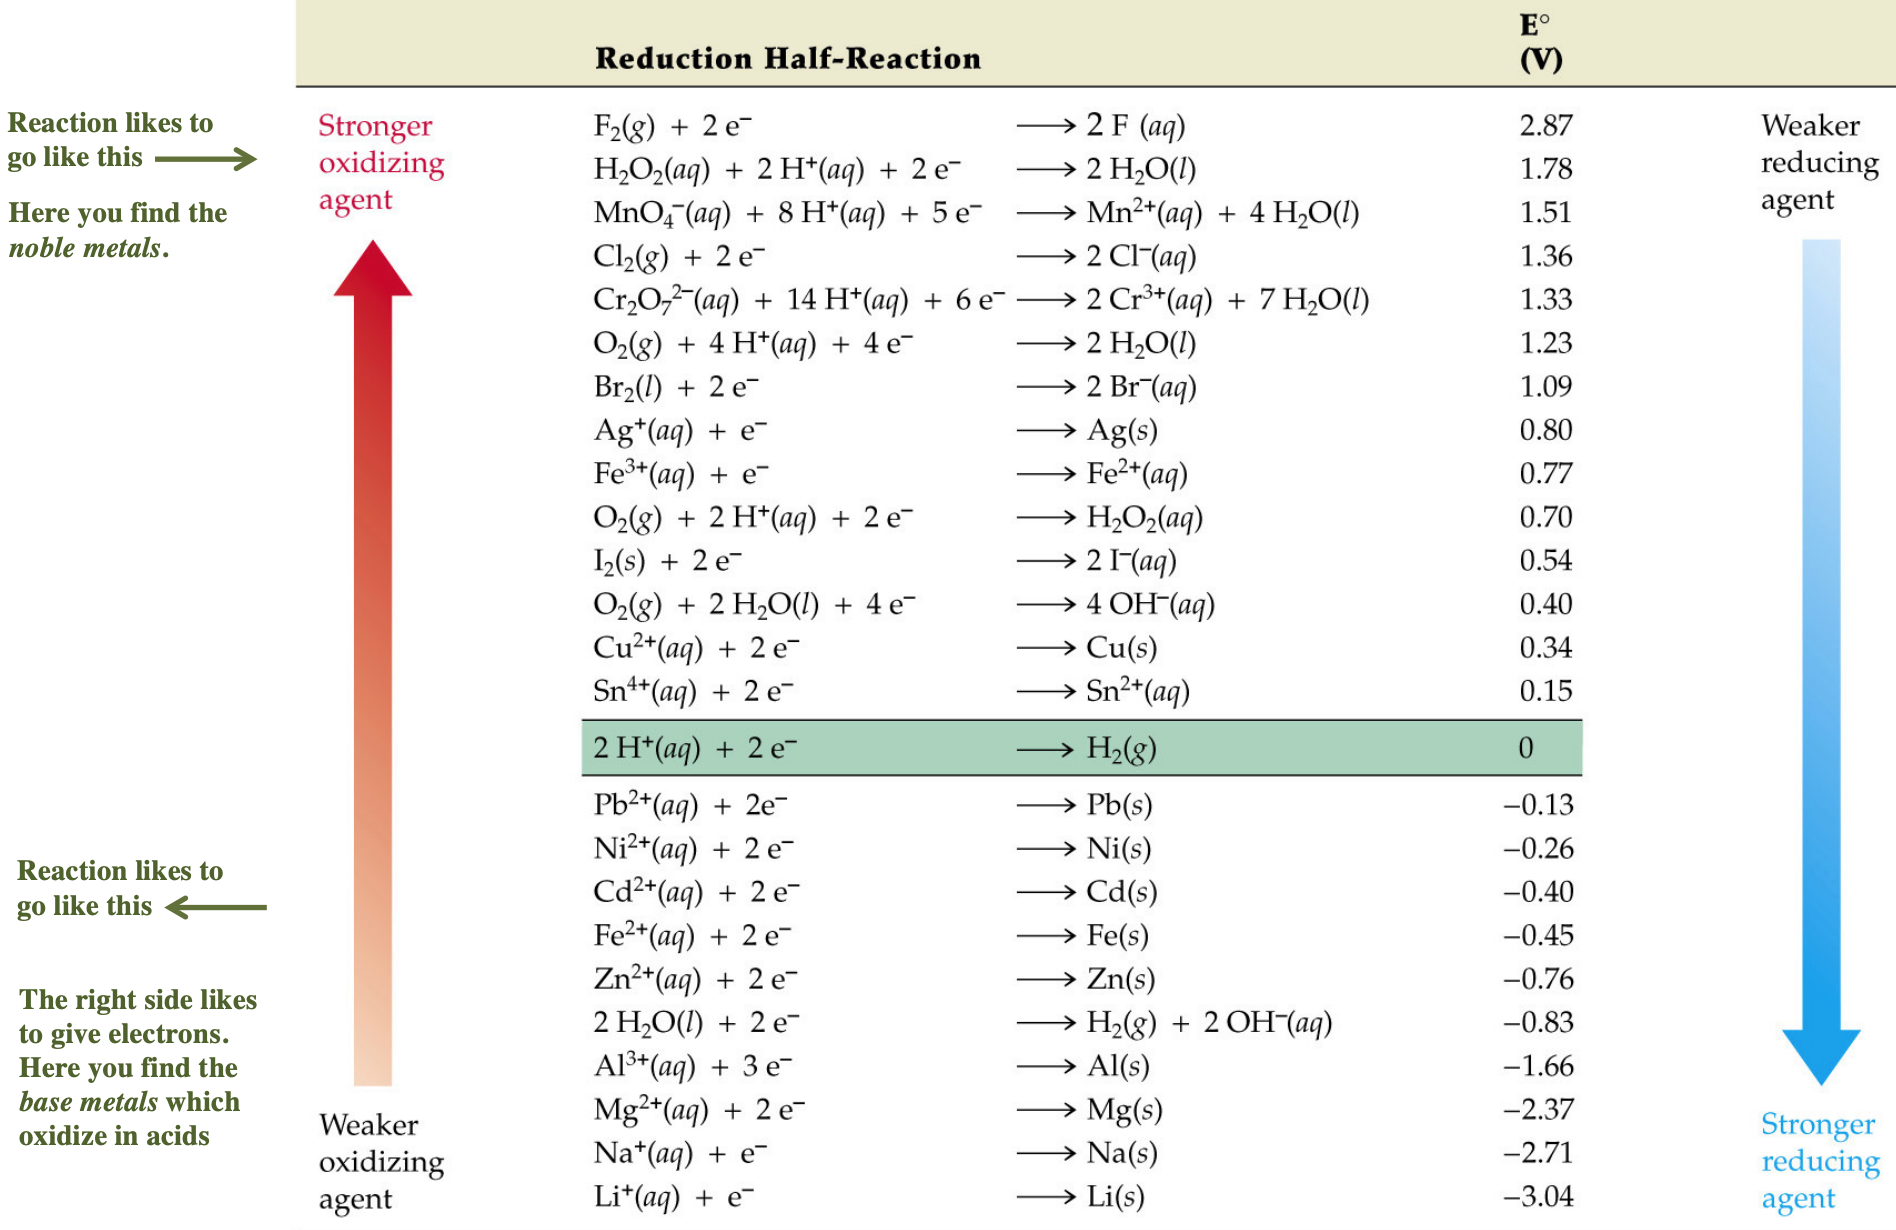
\includegraphics[width=0.8\linewidth]{Something/Images/Small_Redox_Table.png}
        \subsection{Nernst potential at Semipermeable Membranes}
             $j_{diffusion}=-|Z|\cdot D\cdot \frac{d[C]}{dt}$, C: concentration, Z: ion valence, D: diffusion constant \\
             $j_{drift}=-\mu \cdot |Z|\cdot F\cdot [C]\cdot \frac{dV}{dx}$\\
             Einstein relation:  $D=\frac{k_BT\mu}{Q}$\\
             $\implies$ \eqbox{\Delta \varphi = V_{in}-V_{out}=\frac{k_bT}{Q}\cdot \ln {\frac{[C]_{out}}{[C]_{in}}}}\\ 
             $V\cdot c_t(\inf)=V\cdot c_t(0) $\\
             Osmotic equilibrium: $c_1(\inf)=c_2(\inf)$
        \subsection{Ion-Selective Electrodes}
             $\Delta \varphi _m = \frac{RT}{ZF} \ln (\frac{[a_A]_1}{[a_A]_2})$
         
 
        \subsection{Bioenzymatic Sensors}
             \textbf{Enzymes: }lower the activation energy ($E_a$ or $\Delta G$) $\rightarrow$ accelerate the rate of the reaction, are not consumed by the reaction and do not alter the equilibrium of these reactions.\\
            Measure the amount of product after enzymatic reaction to know how much of the reactant was initially present.
        \subsection{ph electrode}
        		$pH=\frac{K'-\Delta\varphi}{0.059}$\\
        Gas sensor CO\textsubscript{2}:\\
        			$H_2CO_3\rightleftharpoons HCO_3^-+H^+$\\
        			$K=\frac{[H^+][HCO_3^-]}{[H_2CO_3]}$\enspace\enspace $pH=pK+ln\frac{[HCO_3^-]}{[H_2CO_3]}$
\section{Amperometric Sensors}
    \textbf{Cathode: }where cations are reduced - gaining charge (electrons are pushed into the electrolyte)\\
    \textbf{Anode: }anions are oxidized - losing charge (electrons are pulled into the circuit)\\
    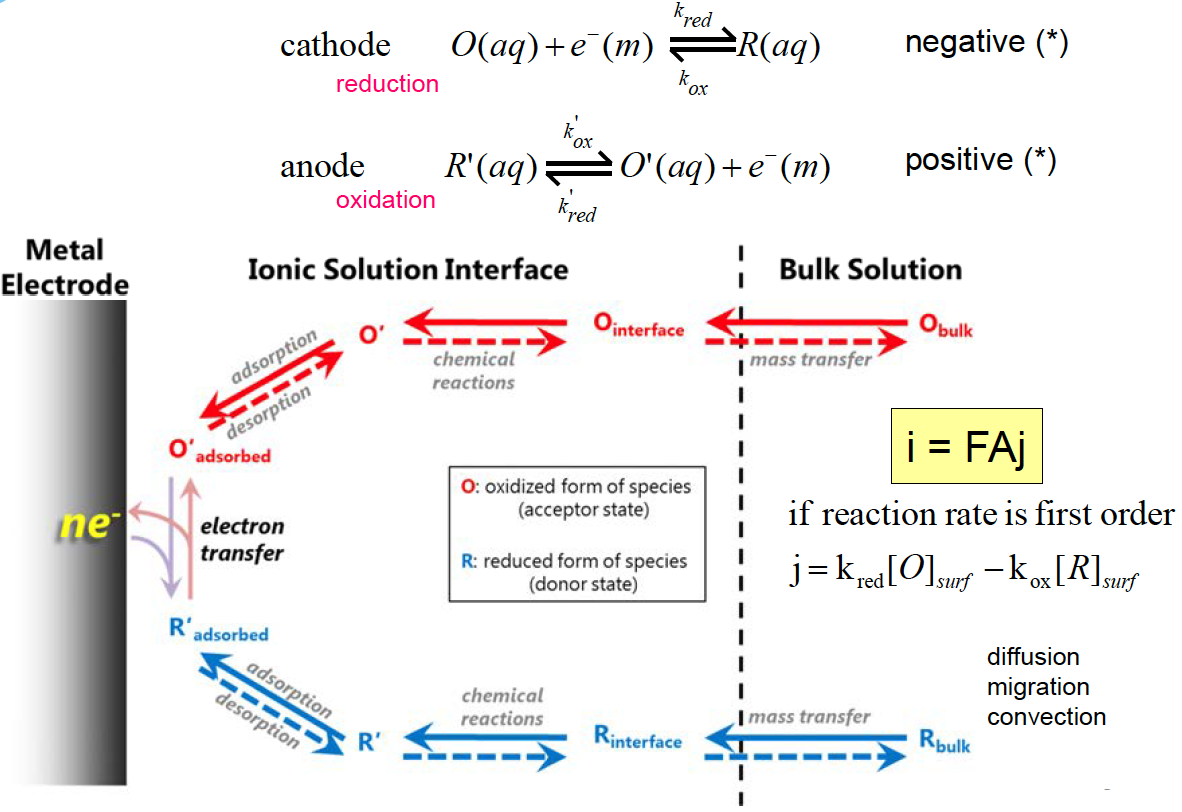
\includegraphics[scale=0.2]{Images/redox_current.png}
        \subsection{Faradays Laws: }
\textbf{First law: }In electrolysis, the quantities of substances involved in the chemical
change are proportional to the quantity of electricity which passes
through the electrolyte. (for every electron, something must have been oxidized)\\
\textbf{Second law: }The masses of different substances set free or dissolved by a given
amount of electricity are proportional to their chemical equivalents. (e.g.  for $X^{2+}$, need 2 electrons to reduce)\\
\textbf{Faradays law of electrolysis: } \\
\eqbox{m=\frac{q\cdot EW }{F}=\frac{i\cdot t\cdot EW}{F}=\frac{Q}{F}\cdot\frac{M}{Z}=\frac{I\cdot t}{F}\cdot\frac{M}{Z}} \\
$EW=\frac{molecular weight}{valency\ 	(z)}$ (see \ref{Faradays law of electrolysis}) \\
	m=mass of substance liberated at an electrode,
		\enspace Q=total electric charge passed through substance,
		\enspace F=Faraday constant,
		\enspace M=molar mass of substance,
		\enspace Z=valency number of ions of the substrate\\
		$n=\frac{I\cdot t}{F}\cdot\frac{1}{Z}$\enspace n=\# of molecules liberated\\
\textbf{Overpotential: }$\eta = \varphi _S - \varphi _M= \Delta \varphi |_{appl} -\Delta \varphi |_{equil} $ \\(find  $\Delta \varphi |_{equil}$ with Nernst equation)\\
$I=\frac{\eta}{R_S}$,\enspace $R_S$=solution resistance
at equilibrium, $\eta =0 \implies k_{ox}=k_{red}= k_0$\\
$k_{red}=k_0 \cdot e^{-n \alpha f \eta}$\\
$k_{ox}= k_0 e^{n(1-\alpha)f\eta}$		(n= number of $e^-$ exchanged)\\
$I=nFAk_0[C_{ox}(0,t)e^{-\alpha n f \eta }-C{red}(0,t)e^{(1-alpha)nf\eta}]$ (i is measured by sensor)


\subsection{Clark electrode}
The Clark electrode is an electrode that measures ambient oxygen concentration in a liquid using a catalytic platinum surface according to the net reactions:\\
Ag (anode): $4Ag^0+4Cl^- \rightarrow 4AgCl+4e^-$ \\
Pt (cathode): $O_2+4e^-+4H^+ \rightarrow 2H_2O$ electrons are pushed into the electrolyte\\
3 types of amperometric sensors:\\
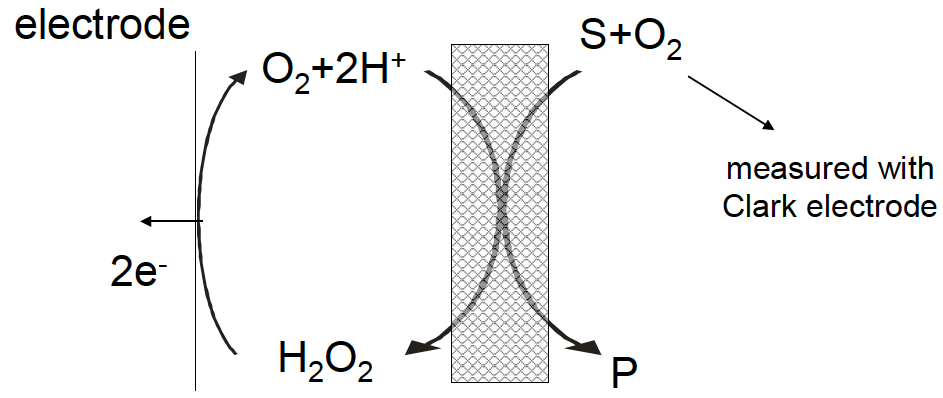
\includegraphics[height=50pt]{Images/O2_based_sensor.png}
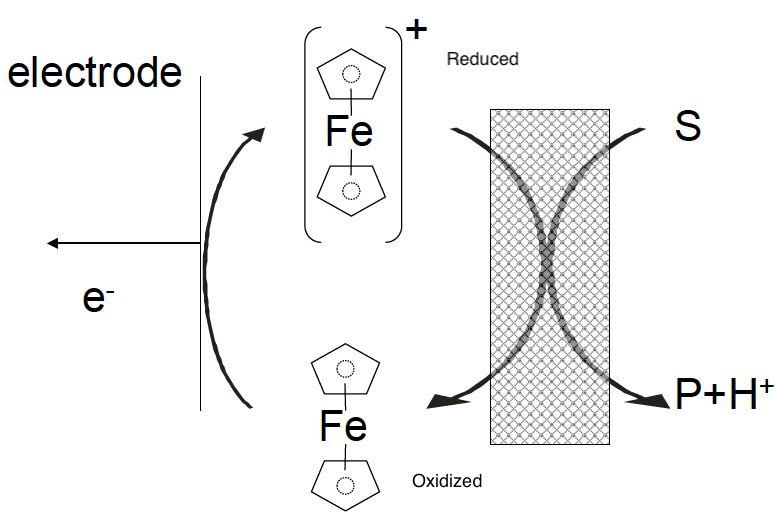
\includegraphics[height=50pt]{Images/mediator_based_sensor.png}
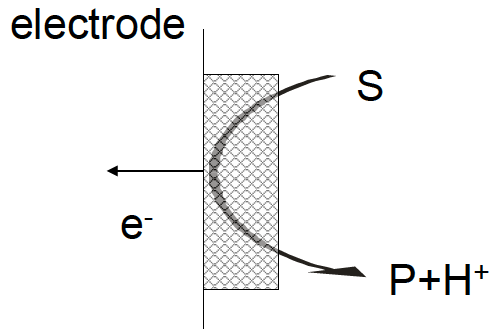
\includegraphics[height=50pt]{Images/Directly-Coupled_Enzymes.png}\\
 (grey rectangle: enzyme)\\
 Problem with directly coupled enzymes: efficiency too low
 \subsection{Energy barrier}
	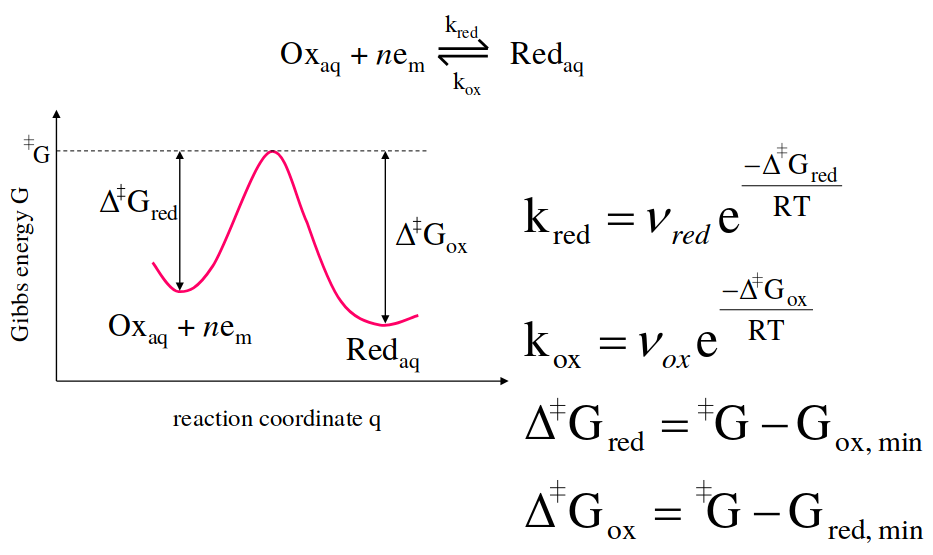
\includegraphics[width=0.8\linewidth]{Images/energy_barrier.png}
		
		\subsection{Butler-Volmer equation}
		\eqbox{i=nFAk_0\left[C_{ox}(0,t)e^{-\alpha nf\eta}-C_{red}(0,t)e^{(1-\alpha)nf\eta}\right]}\\
		$n=\#$ of $e^-$ exchanged,
		\enspace $\eta=\text{overpotential}$,
		\enspace $f{=}\frac{F}{RT}$,\\
		\enspace $F=\text{Faraday const.}$,
		\enspace $R=\text{gas const.}$,
		\enspace $A=\text{surface area of electrode}$,\\
		\enspace $\alpha=\text{transfer coefficient}$,
		\enspace $C_{ox}/C_{red}$=concentration of oxidant/reductor
 
 
 \section{Membranes and Transport}
    concentration=$c(x,t)\enspace \left[\frac{mol}{cm^3}\right]$\enspace\enspace\enspace$1L=10^3cm^3$\\
    flux=$\phi(x,t)\enspace \Big[\frac{mol}{cm^2\cdot s}\Big]$\enspace\enspace\enspace$1M=10^{-3}mol/cm^3$\\
    \textbf{Ficks law of Diffusion: }$\phi (x,t)=-D\frac{\partial c(x,t)}{\partial x}$\\
    \textbf{Continuity equation: }$-\frac{\partial \phi (x,t)}{\partial x}=\frac{\partial c(x,t)}{\partial t}$\\
    \textbf{Steady state: }$\frac{\partial \phi (x,t)}{\partial t}=0 \implies -D\frac{\partial c(x,t)}{\partial x} =const \rightarrow c(x,t)=c(x,t_0)$
    \textbf{Equilibrium: }$\phi(x,t)=0$\\
    Total amount of substrate in both compartments must remain the same: $C_1(0)A_1L_1+C_2(0)A_2L_2=C_1(\inf )A_1L_1+C_2(\inf )A_2L_2$
    \subsection{Membrane Diffusion}
        Extremely fast establishment of equilibrium in membrane\\
        \textbf{Ficks law for membranes: }\\$\phi _n(t) [\frac{mol}{cm^2\cdot s}]=P_n(c_n^i(t)-c_n^0(t))$; $P_n=\frac{D_n\cdot k_n}{d}$\\
        			\enspace $P_n$=permeability of membrane to solute n,
			\enspace $\phi_n(t)$=flux through membrane,
			\enspace $c_n^i(t)$=concentration inside,
			\enspace $c_n^o(t)$=concentration outside,
			\enspace $d$=thickness of membrane,
			\enspace $D_n$=diffusion constant,
			\enspace $k_n$=partition coefficient, example:$k_{oil:water}=\frac{c_n^{oil}}{c_n^{water}}$
    \subsubsection{Osmosis}.\\
        Movement of solvent/water across membranes\\
        Osmosic Pressure: \eqbox{\pi (x,t)=RT\sum _n C_n(x,t)} (Van't Hoff's law)\\
        There is diffusion across the membrane until $\pi (x,t)=0$
        $\pi(x,t)=\text{osmotic pressure}\Big[Pa=\frac{N}{m^2}\Big]$,\\
		$C_{\sum}(x,t)=\mathrm{osmolarity}\Big[\frac{osmol}{m^3}\Big]$,\\
		$R=\text{molar gas constant}=8.314J/mol\cdot K$\\\\
    

	\subsection{Carrier mediated transport}
	Carrier mediated transport saturates (elevator analogy), works by competition and is structure dependent/ not formula dependent\\
        Binding $\rightarrow$ translocation $\rightarrow$ release $\rightarrow$ reset \\
        Number of substrates in a state: $\eta ^{i,o}_{E,ES}$ (i/o for inside or outside facing, E/ES for with/without substrate)\\
		4-state carrier model:\\
		\begin{wrapfigure}[10]{l}{0.5\linewidth}
		\vspace{-20pt}
		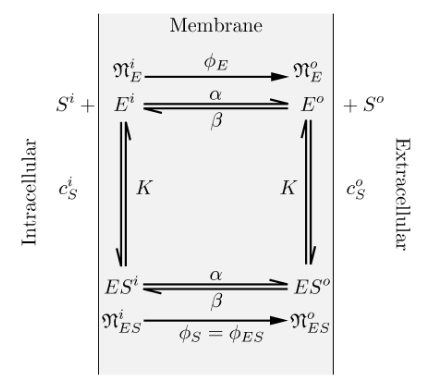
\includegraphics[width=\linewidth]{Images/4-state_carrier_model.png}
		
		\end{wrapfigure}
		$\mathfrak{R}_{ES}^i=\Big(\frac{\beta}{\alpha+\beta}\Big)\Big(\frac{c_S^i}{c_S^i+K}\Big)\mathfrak{R}_{ET}$\\
		$\mathfrak{R}_E^i=\Big(\frac{\beta}{\alpha+\beta}\Big)\Big(\frac{K}{c_S^i+K}\Big)\mathfrak{R}_{ET}$\\
		$\mathfrak{R}_{ES}^o=\Big(\frac{\alpha}{\alpha+\beta}\Big)\Big(\frac{c_S^o}{c_S^o+K}\Big)\mathfrak{R}_{ET}$\\
		$\mathfrak{R}_E^o=\Big(\frac{\alpha}{\alpha+\beta}\Big)\Big(\frac{K}{c_S^o+K}\Big)\mathfrak{R}_{ET}$\\
		net flux out of cell:\\$\phi_s{=}\Big(\frac{\alpha\beta}{\alpha+\beta}\Big)\mathfrak{R}_{ET}\Big(\frac{c_S^i}{c_S^i+K}{-}\frac{c_S^o}{c_S^o+K}\Big)$\\
		\\
		with $\phi _S=\phi _{ES} = \alpha \eta _{ES}^i - \beta \eta_{ES}^o$ and $\eta _{ET}$ the total amount of enzymes
	   \subsection{Ion transport}
		Nernst Potential:\\\eqbox{\Delta\Psi_{12}=\Psi_1-\Psi_2=\frac{D_n}{u_nz_nF}ln\Big(\frac{c_2}{c_1}\Big)=\frac{RT}{z_nF}ln\Big(\frac{c_2}{c_1}\Big)}\\
		Nernst equilibrium potential:\\\eqbox{V_m=\frac{RT}{z_nFlog_{10}(e)}log_{10}\Big(\frac{c_S^o}{c_S^i}\Big)}, At 300K, $v_n \approx \frac{60}{z_n}\log (\frac{c_n^o}{c_n^i})$mV\\\\
		Multiple-ion model:\\
		\begin{wrapfigure}[6]{l}{0.25\textwidth}
		\vspace{-20pt}
			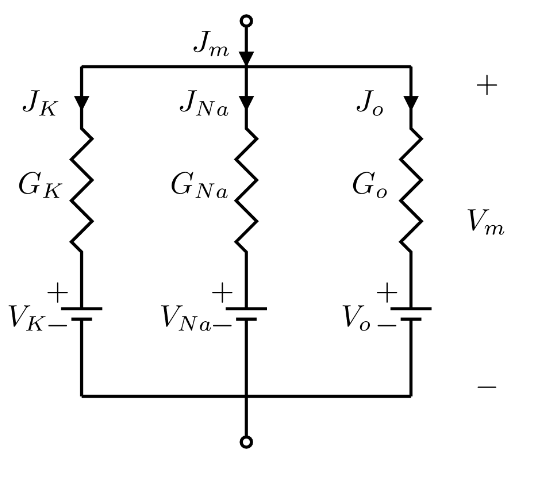
\includegraphics[width=0.7\linewidth]{Images/multiple-ion_model.png}\\
		\end{wrapfigure}
	
		at steady state:\\
		$J_{Na}{+}J_K{+}J_o=0$\\
		$J_m=0$\\
		$V_m{=}\frac{V_{Na}G_{Na}}{G_{tot}}{+}\frac{V_KG_K}{G_{tot}}{+}\frac{V_oG_o}{G_{tot}}$\\
		$J_{NA/K}=G_{NA/K}(V_m-V_{NA/K})$\\
		\\\\
		.\\
Potassium is the dominant ion (highest conductance), sodium has only a small effect, all other ion lumped together in $V_0,G_0$\\
		\subsection{active transport}
		-add active pump for each ion to keep net ion current zero
		-now we have both $J_m=0$ and quasi-equilibrium $J_n^a+J_n^p=0$ 
	
		
\section{Action potential \& Hodgkin and Huxley Model}
		"Clamp" refers to keeping a parameter constant. In \textbf{current clamp}, the current passing across the membrane is controlled experimentally, and the membrane voltage changes that take place are measured. In \textbf{voltage clamp}, the membrane voltage is controlled experimentally, and the current passing across the membrane is measured.
		\subsection{Hodgkin Huxley Model}

			 state variables:$V_m(t),n(t),m(t),h(t)$\\
			state equations:
			\\\boxed{\begin{aligned}
			&\tau_n(V_m)\frac{dn(V_m,t)}{dt}+n(V_m,t)=n_{\infty}(V_m)\\
			&\tau_m(V_m)\frac{dm(V_m,t)}{dt}+m(V_m,t)=m_{\infty}(V_m)\\
			&\tau_h(V_m)\frac{dh(V_m,t)}{dt}+h(V_m,t)=h_{\infty}(V_m)\\
			&G_K(V_m,t)=\bar{G}_Kn^4(V_m,t)\\
			&G_{Na}(V_m,t)=\bar{G}_{Na}m^3(V_m,t)h(V_m,t)
			\end{aligned}}
			\boxed{
			\begin{aligned}
	            &\text{initial conditions:}\\
	            &V(t=0)=V_m^0,\\
	            &n(t=0)=n_{\infty}(V_m^0),\\
	            &m(t=0)=m_{\infty}(V_m^0),\\
	            &h(t=0)=h_{\infty}(V_m^0)
			\end{aligned}
			}\\
			$J_m(t)=J_C+J_{Na}+J_K+J_L+J_{ext}=\\C_m\frac{dV_m(t)}{dt}+G_{Na}(V_m,t)
			\cdot(V_m(t)-V_{Na})+G_K(V_m,t)\cdot(V_m(t)-V_K)+G_L\cdot(V_m(t)-V_L)+J_{ext}
			=0$\\
			\boxed{
			\begin{aligned}
				&\alpha_m=\frac{-0.1(V_m+35)}{e^{-0.1(V_m+35)}-1}K_T\\
				&\beta_m=4e^{-(V_m+60)/18}K_T\\
				&\alpha_h=0.07e^{-0.05(V_m+60)}K_T\\
				&\beta_h=\frac{1}{1+e^{-0.1(V_m+30)}}K_T\\
				&\alpha_n=\frac{-0.01(V_m+50)}{e^{-0.1(V_m+50)}-1}K_T\\
				&\beta_n=0.125e^{-0.0125(V_m+60)}K_T
			\end{aligned}
			}
            \boxed{
			\begin{aligned}
				\tau_m=\frac{1}{\alpha_m+\beta_m} , m_{\infty}=\frac{\alpha_m}{\alpha_m+\beta_m}\\
				\tau_h=\frac{1}{\alpha_h+\beta_h} , h_{\infty}=\frac{\alpha_h}{\alpha_h+\beta_h}\\
				\tau_n=\frac{1}{\alpha_n+\beta_n} , n_{\infty}=\frac{\alpha_n}{\alpha_n+\beta_n}	
			\end{aligned}
			}\\
			Standard parameters:$\bar{G}_{Na}=120,\bar{G}_K=36, G_L=0.3mS/cm^2,\\C_m=1\mu F/cm^2,c_{Na}^o=491, c_{Na}^i=50,
			c_{K}^o=20.11,c_K^i=400 mmol/L, \\V_L=-49mV, temperature=6.3^\circ C$\\
		temperature factor:$K_T=3^{(T_C-6.3)/10}$\\
		\textbf{higher temperature: }- action potential dynamics will be faster and amplitude
        will get smaller. 
        - reduces the amplitude of the sodium conductance relative to
        the potassium conductance at the peak of the action potential\\
        And for \textbf{low temperatures} the action potential
dynamics will get slower and will not fire that frequently.
		$V_n=\frac{R(T_C+273.16)}{z_nF}ln\Big(\frac{c_n^o}{c_n^i}\Big)$
	
		
		
		\subsection{Action Potential}
		\textbf{Properties of Action Potential: }\\
- \textbf{All-or-none}\\
- \textbf{Refractoriness}: After the AP generation, it is more difficult to generate APs\\
- \textbf{Strength duration relation}: For longer duration current
pulse, the lower the current
threshold for stimulation of
AP.\\
- \textbf{Decrement-free conduction}\\
- \textbf{Accomodation}: For slow enough ramp-up of current, axon "accomodates" and does
not generate action potential (even at above the threshold).\\
-\textbf{ Anode break}: By hyperpolarizing (going more negative) and then repolarizing back to
resting potential, you could elicit action potential as well.\\
\textit{It is a change in conductance through the ion channels by opening of 4 charged gates that enables the AP}\\
open-channel probability x(Vm) goes up as Vm $\uparrow$\\
$G_K$: 4 independent gates\\
$G_{NA}$: 3 (fast -higher positively charged) activating gates + 1 (slowly -low negatively charged) inactivating gate

		4 regimes during AP:\\

		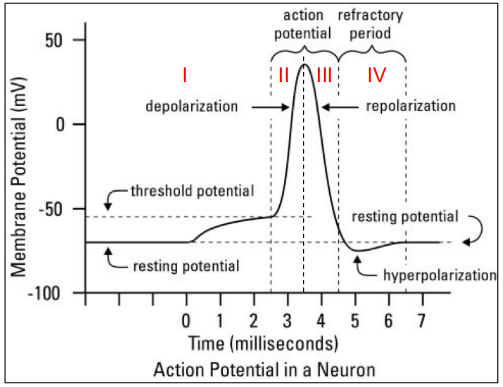
\includegraphics[width=0.8\linewidth]{Images/AP.png}

		I:Pre-AP threshold\\
		II:AP initiation\\
		III:AP ending\\
		IV:Post-AP refractory period\\
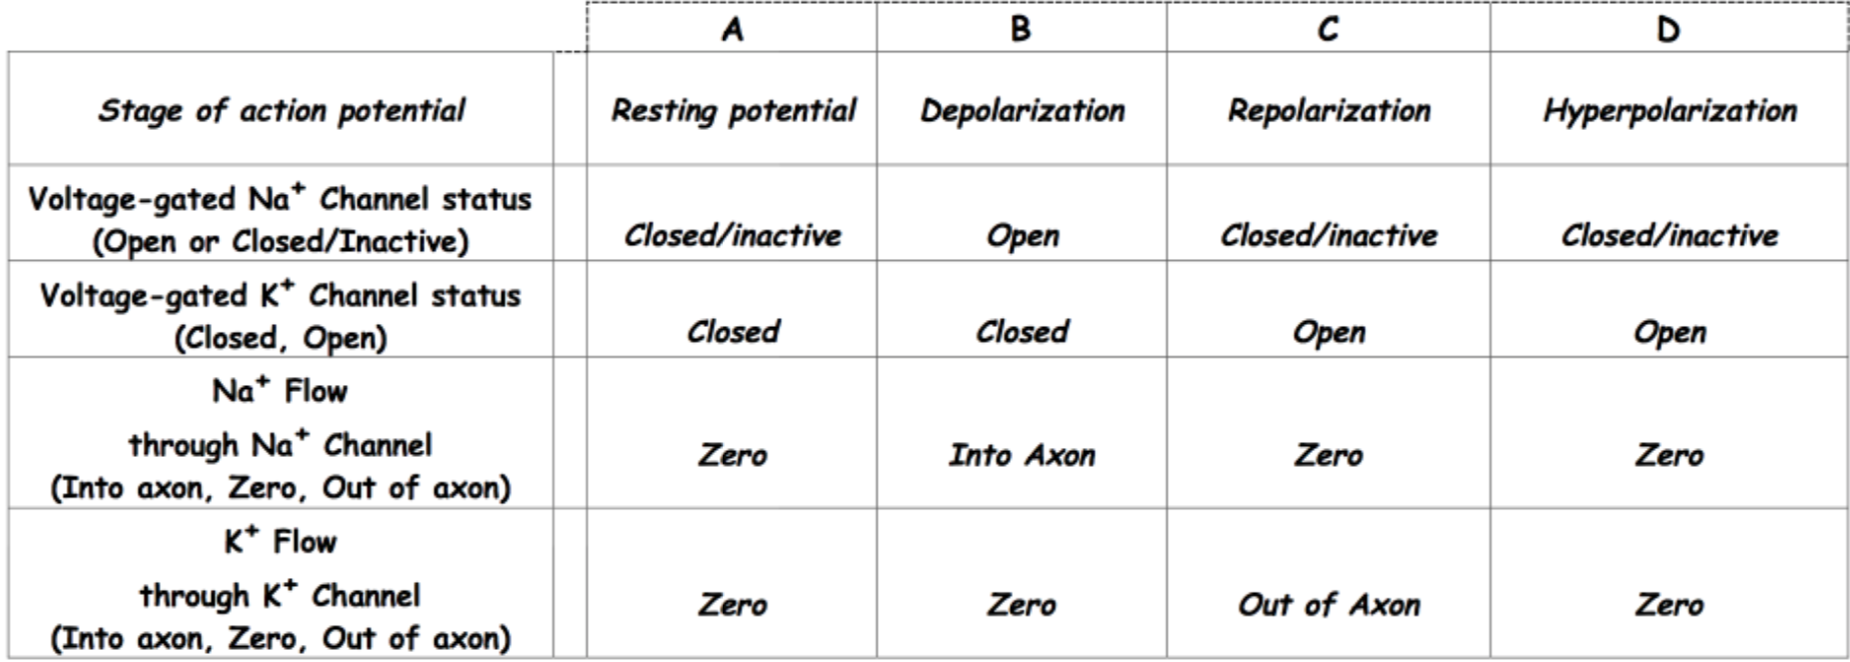
\includegraphics[width=0.8\linewidth]{Something/Images/sodium_potassium_gates.png}\\
		\textbf{Resting Potential of neuron: }results from a higher concentration of sodium on the outside and a higher concentration of potassium on the inside due to the \emph{Sodium-Potassium pump}. In total there is a higher concentration of positive charges on the outside than on the inside.\\
		\textbf{Node of Ranvier: }a natural gap in the myelin sheath along the axon. These unmyelinated spaces are about one micrometer long and contain voltage gated Na+ and K+ channels. The flow of ions through these channels, particularly the Na+ channels, slows the action potential down but regenerates it over and over again along the axon.		
\section{Core conductor model}

The speed of conduction is improved with a myelin sheet (keeps current in axons) and the AP is regenerated through the nodes of Ranvier\\ 
		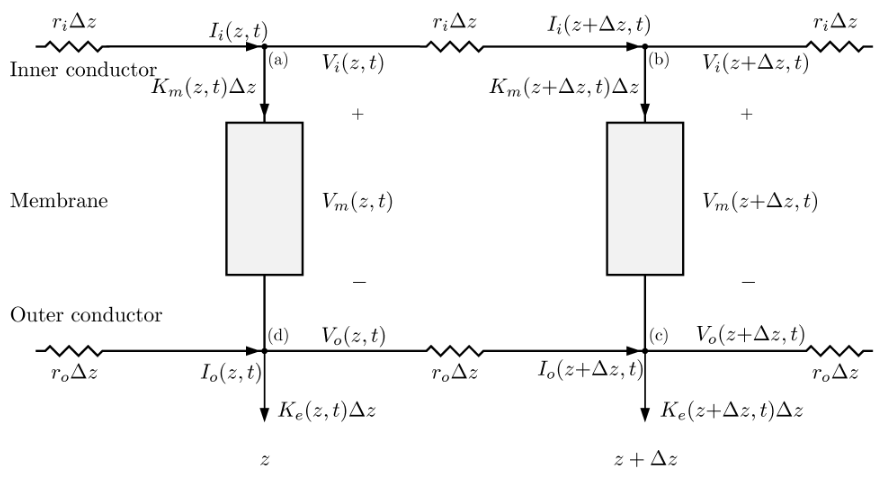
\includegraphics[width=0.8\linewidth]{Images/core-conductor.png}
		\\
		\boxed{
		\begin{aligned}
			&\frac{\partial I_i(z,t)}{\partial z}=-K_m(z,t)\\
			&\frac{\partial I_o(z,t)}{\partial z}=K_m(z,t)-K_e(z,t)\\
			&\frac{\partial V_i(z,t)}{\partial z}=-r_iI_i(z,t)\\
			&\frac{\partial V_o(z,t)}{\partial z}=-r_oI_o(z,t)
		\end{aligned}
		}\\
		$r_i$=inner resistance per unit length\\
		$r_o$=outer resistance per unit length\\
		$K_m$=current per unit length\\
		$K_e$=external current that is applied\\
		$V_m(z,t)=V_i(z,t)-V_o(z,t)$
		\\
		$\frac{\partial V_m(z,t)}{\partial z}=-r_iI_i(z,t)+r_oI_o(z,t)$\\
		\eqbox{\frac{\partial^2V_m(z,t)}{\partial z^2}=(r_o+r_i)K_m(z,t)-r_oK_e(z,t)}\\
		velocity of AP: $v=\sqrt{\frac{K_m}{(r_i+r_o)2\pi a}}\approx\sqrt{\frac{K_m a}{2\rho_i}}$\\
		$\rho_i$=resistivity\\
		cable equation:\\\eqbox{v_m+\tau_m\frac{\partial v_m}{\partial t}-\lambda_c^2\frac{\partial^2 v_m}{\partial z^2}=r_o\lambda_c^2K_e}\\
		$\lambda_c{=}\frac{1}{\sqrt{g_m(r_o+r_i)}}$

		\section{Functional stimulation and recording}
		\begin{wrapfigure}[10]{l}{0.3\linewidth}
		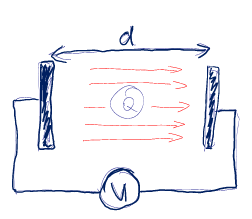
\includegraphics[width=0.7\linewidth]{Images/E-field.png}\\
		\end{wrapfigure}
		$E=\frac{U}{d}$\\
		$F=Q\cdot E$\\
		$\frac{1}{R}=\frac{I}{U}=\frac{I}{Ed}=\frac{A}{d}c_{ion}\lambda_{mol}$\\
		$F=zeE$,$v=\frac{z\cdot e \cdot \mu}{A\cdot c_{ion}\lambda_{mol}}$\\
		
		Double layer capacitance of cell: $C{=}\frac{Q}{\Psi_o}{=}{-}\frac{Dze}{4\pi kT}\kappa A$\\
		\\
		total capacitance of cell:\\$\frac{1}{C_{total}}=\frac{1}{C_{dl,in}}+\frac{1}{C_{stem,in}}+\frac{1}{C_{membrane}}+\frac{1}{C_{stem,out}}+\frac{1}{C_{dl,out}}$	
	
	
	
	
	
	
	
	
	\section{Formulas}                 
\subsection{Mechanical waves}
Speed: $c = 1/\sqrt{\kappa\rho}$; P: $p = \rho c u_z$;
Impedance: $Z = p/u_z = \rho c = \sqrt{\rho/\kappa}$; Intensity: $I = p u_z/2$; WL: $\lambda = {c/\nu} = {1/(\nu \sqrt{\kappa \rho})}$; Part.vel: $u_z=\sqrt{2I/Z}$

\subsection{Basic Physics}

	\begin{tabular}{lll}
	photon energy $[J]$									&$E$      &$hc/\lambda$\\
		arc length          										&$s$    &$=\frac{\pi \cdot r\cdot \theta}{180}$\\
		Force $[kg\cdot m \cdot s^{-1}]$                 & $F$       & $=m \cdot a=Q\cdot E$ \\
		Work $[kg\cdot m^2\cdot s^{-2}]$                & $W$       & $=F\cdot s = \int _{t_{1}}^{t_{2}}\mathbf {F} \cdot \mathbf {v} dt$ \\ 
						&		   &$=\int _{C}\mathbf {F} \cdot d\mathbf {s}$                                        \\
		Power $[kg \cdot m^2 \cdot s^{-3}]$               & $P$       & $=\frac{\Delta W}{\Delta t}= F\cdot v$                                       \\
				       &           & $=R\cdot I^2=V\cdot I$                            \\
		Momentum           & $p$               & $=mv=\sqrt{2 E m}$ \\
		Electric Field			&$E$				&$=\frac{U}{d}$\\
		Kinetic energy     & $E_{kin}$ & $=\frac{1}{2}mv^2$                                \\
		Impulsenergie         & $E_{kin}$ & $=\frac{p^2}{2m}$                                 \\
		Potentielle Energie    & $E_{pot}$ & $=mgh$                                            \\
		Eletrische Energie     & $E_{el}$  & $=e\cdot V_0$                                     \\
		Modell freies Elektron & $E$       & $=\frac{\hbar^2}{2m^*}k^2$                        \\
		Spannungsenergie       & $E_{pot}$ & $=\frac{1}{2}mx^2$                                \\
		Federkraft             & $F$       & $=-kx$                                            \\
		Gravitationskraft      & $F_G$     & $=G\frac{m_1m_2}{r^2}$    
		\\
		Gravitational Potential Energy & $V_G$  & $=-G\frac{m_1m_2}{r}$ 
		\\
	\end{tabular}
\subsection{Conversions}

		$\text{Power in dB= }10\cdot log(\frac{I}{I_0})\\
		\text{Faraday Constant F= }eN_a=9,6485\cdot 10^4 C\cdot mol^{-1}\\
		\text{Gas constant R= }8.31 \frac{J}{mol\cdot K}\\
		\text{Num Avogadro } N_A=  6.022\cdot 10^{23}\ mol^{-1}\\
		$Boltzmann constant $k_B=\ 1.380658\cdot 10^{-23}\ J/K = 8.6\cdot 10^{-5}\ eV/K\\ 
		\text{Newton: }\SI{1}{\newton}=\si{\kilo\gram\meter\per\square\second}\\
		\text{Pascal: }\SI{1}{\pascal}=\si{\newton\per\meter}\\
		\text{Joule: }\SI{1}{\joule}=\si{\newton\meter}=\si{\kilo\gram\square\meter\per\square\second}=\SI{6.2415e18}{\electronvolt}\\
		\text{Watt: }\SI{1}{\watt}=\si{\kilo\gram\square\meter\per\cubic\second}\\
		\text{Angström: } \SI{1}{\angstrom} = \SI{0.1}{\nano\meter}$
	
\subsubsection{Trigonometric conversions}.\\
$
	\sin(\alpha)\cos(\beta) = \frac{1}{2}(\sin(\alpha+\beta)+\sin(\alpha-\beta))                     \\
	\cos(\alpha)\cos(\beta)  = \frac{1}{2}(\cos(\alpha+\beta)+\cos(\alpha-\beta))                     \\
	\sin(\alpha)\sin(\beta)  =\frac{1}{2}(\cos(\alpha-\beta)-\cos(\alpha+\beta))       $

\subsection{Stuff}
\subsubsection{Harmonic Oscillator}.\\
Average work done in one cycle ($T= \frac{2\pi}{\omega}$) $\bar{W}= \frac{1}{T} \int _{0}^{T} \vec{F} \cdot \vec{x}\ dt$\\
Average Power: $\bar{P}= \frac{\bar{W}}{T}$\\
\subsubsection{Beer-Lambert}.\\
$A=\epsilon\cdot l\cdot c=-log_{10}(I/I_0)$\\
\subsubsection{pH}.\\
pH$= -\log [H^+] =-\log [H_3 O^+] $ in water\\
\subsubsection{Faradays law of electrolysis} \label{Faradays law of electrolysis}.\\
$\Delta Q= z\cdot F\cdot \Delta [ion]\cdot V$\\
relates the amount of material produced at an electrode during an electrochemical reaction to the total charge passed or, equivalently, the average current and total time.\\
$n=\frac{Q}{F\cdot z}$
\subsubsection{Ideal Gas law}.\\
$PV=nRT$\\
\subsubsection{Stoke's law}.\\
The force of viscosity on a small sphere moving through a viscous fluid is given by:\\
 \grey{$F_{d}=6\pi \,\eta \,R\,v\  (= z\, e\, E=\frac{v}{\mu})$}\\
$F_d$ is the frictional force acting on the interface between the fluid and the particle\\
$\eta $ is the dynamic viscosity \\
R is the radius of the spherical object\\
$v$ is the flow velocity relative to the object\\
$\mu$ being the mobility\\
\subsubsection{Einstein Relation}.\\
Duffusion constant: $D= \mu \,  k_B\, T$\\
Electrical mobility equation: $\frac{\mu \, k_b\, T }{q}$\\
Stokes-Einstein equation: $D=\frac{k_b\, T}{6\pi \,\eta \,R}$\\
\subsubsection{Conductivity of ionic solutions}.\\
$\frac{1}{R}=\frac{A}{d}\, C_{ion}\, \lambda _{mol}=\frac{I}{E\cdot d}$, 
with $\lambda {mol}$ the molar conductivity
\end{multicols}


\end{document}